\documentclass[12pt]{mitthesis} 

\usepackage{lgrind, braket, amsmath, paralist,
  amssymb, bbm, booktabs, subfig, color} 

\usepackage[pdftex]{graphicx}
\usepackage[version=3]{mhchem}

\newcommand{\TODO} [1]{\textcolor{magenta}{\textbf{TODO:} #1}}
\newcommand{\NOTE} [1]{\textcolor{magenta}{[\emph{#1}]}}
\newcommand{\POINT}[1]{\textcolor{magenta}{\textbf{POINT:} #1}}

\newcommand{\rcm}{cm$^{-1}$}
\newcommand{\bigspace}{$
  \;
  $}

\newcommand{\astate}{$
  \tilde{A} \: ^1\!A_u
  $}
\newcommand{\AtoX}{$
  \tilde{A} \: ^1\!A_u 
  \leftarrow 
  \tilde{X} \: ^1\Sigma_g^+
  $}
\newcommand{\StoS}{$
  S_1 \leftarrow S_0
  $}
\newcommand{\microsec}{$\mu$s}

\newcommand{\Ka}[1]{$K_a\!\!=\!#1$}

% scientific notation
\newcommand{\e}[1]{\ensuremath{\times 10^{#1}}}

% temperatures
\newcommand{\degrees}{\ensuremath{^\circ}}



% hyphenation
\hyphenation{acetylene}
\hyphenation{Hamiltonian}

\begin{document}

\tableofcontents
\clearpage

\listoffigures
\clearpage

\subsubsection*{NOTES}

\clearpage

\setcounter{chapter}{3}
\chapter{SEELEM/LIF spectroscopy of acetylene: Spectral signatures of
  energetically distant doorway levels}

% \section{Introduction}

% What are the global characteristics of doorway-mediated intersystem
% crossing in acetylene,\ce{C2H2}?  \TODO{Trash and rewrite the entire
%   paragraph.}  The dynamics of singlet$\sim$triplet coupling in the
% \AtoX \bigspace (\StoS) electronic spectrum of acetylene, \ce{C2H2},
% have been extensively studied.  This body of work establishes a
% heirarchical model for electronic coupling, which leads to the effects
% of intersystem crossing and internal conversion: $S_1 \rightarrow T_3
% \rightarrow T_{1,2} \rightarrow S_0$.  Top-tier interactions between
% the relatively sparse levels of the $S_1$ and $T_3$ electronic states
% are of particular interest because (1) they control coupling to the
% remaining electronic states of the molecule and (2) they are primarily
% determined by vibrational overlap factors and energy denominators, two
% sensitive consequents of the molecule's electronic structure.

% % Singlet~triplet coupling in the S_1 state of trans-acetylene is
% % mediated by the relatively sparse (0.1 per cm-1) levels of the third
% % triplet state, T_3.  When a mediating T_3 level is energetically
% % distant from an interacting singlet level, traces of its influence
% % appear in the patterns of coupling between the singlet level and the
% % dense, local manifold of T_1,2 levels (10 per cm-1).  The method of
% % SEELEM spectroscopy is tuned to detect molecules in such second-tier
% % eigenstates, being most sensitive to states with about 0.1\% S_1
% % character.  Conversely, LIF spectroscopy is sensitive to molecules in
% % states with large amounts of S_1 character.

% Surface Electron Ejection by Laser-Excited Metastables \cite{sneh89a,
%   sneh89b, sneh91, humphrey97} (SEELEM) and LIF spectroscopy are
% complementary techniques, which, when used together, can provide
% information about $S_1 \sim T_3$ interactions \cite{humphrey97,
%   mishra04, altunata00, altunata02}.  \TODO{Finish adapting from
%   paper.}  LIF detection is limited to short-lived
% ($\tau_{radiative}<$ 10 \microsec), strongly fluorescing states, while
% SEELEM detection is sensitive only to long-lived ($\tau >$ 300
% \microsec) states with vertical electronic excitation above a
% threshold energy set by the work function of the metal used as the
% SEELEM detector surface.  Therefore, SEELEM and LIF detection channels
% observe mutually exclusive sets of eigenstates that arise from
% spin-orbit mixed $S_1$ and $T_{3,2,1}$ zero-order basis states.
% Because SEELEM detection is sensitive to the electronic character of
% the molecule, a comparison of simultaneously recorded SEELEM and LIF
% spectra reveals features of electronic structure and photochemical
% pathways that are invisible via traditional, single-channel
% spectroscopic probes such as LIF alone, REMPI, phosphorescence, or
% phosphor surface \cite{shi98, campos01, burton72}.
 
% % Information gained from comparison of acetylene SEELEM
% % and LIF spectra can yield a mechanistic description of
% % singlet$\sim$triplet interaction, and holds promise for describing the
% % structure and dynamics of other small polyatomic species \cite{jung07,
% %   allen07}.
% % SEELEM spectroscopy has
% % been used in this effort as a tool to examine $S_1 \sim T_3$ coupling,
% % by allowing detection of the local manifold of predominantly $T_{1,2}$
% % eigenstates in the region surrounding an \StoS\ transition.

% The \emph{trans}-bending mode of $S_1$ acetylene, $\nu_3$, is known to
% be an important promoter of singlet$\sim$triplet coupling.  In Zeeman
% anticrossing experiments, Dupr\'{e} and coworkers observed a rapid
% increase in the anticrossing density, as well as the product
% $\rho_{\text{vib}} \braket{H_{st}}$, with energy in $\nu_3$
% \cite{dupre91, dupre95b}.  They also observed an single large
% singlet$\sim$triplet anticrossing in the $3 \nu_3$ $K_a=0$ level,
% %with a zero-field matrix element of 0.29 \rcm,
% which was in turn perturbed by many smaller couplings \cite{dupre93}.
% These observations led the authors to propose that the
% singlet$\sim$triplet dynamics of acetylene in the \astate\ state are
% best described by a doorway-mediated mechanism, in which particular
% triplet vibrational levels mediate intersystem crossing between the
% initially excited $S_1$ bright state and the dense manifold of highly
% mixed, dark $T_{1,2}$ states.  Subsequent theoretical and experimental
% work confirmed that the coupling doorways were vibrational levels of
% the $T_3$ electronic state \cite{vacek96, sherrill96, humphrey97,
%   altunata00}.

% The $S_1$ $3 \nu_3$ $K_a$=1 level has been heavily studied due to a
% local $S_1 \sim T_3$ level crossing at $J \approx 3$.  Spectroscopic
% patterns in SEELEM arising from the effects of the local $T_3$
% perturber in have been discussed by several authors \cite{humphrey97,
%   altunata00, altunata01, mishra04}.  Using vibrational overlap
% integrals gained from \emph{ab initio} calculations of the $T_3$
% electronic surface, Thom and coauthors were able to exclude all but
% several candidate $T_3$ levels as the $3\nu_3$ local perturber
% \cite{thom07}.
% % \POINT{Overlap between $S_1$ and $T_3$ levels predicted by Bryan and
% %   Ryan.  (See p.40 of 1/2007--3/2007 notebook.)}
% However, recent observations of an increase in average $T_{1,2}$
% electronic character at higher values of $J$ suggest that the local
% $T_3$ perturber is not the sole, and perhaps not the primary, doorway
% for $3 \nu_3$ \cite{degroot07}.

% That an energetically distant doorway, which would be required to have
% a correspondingly larger spin-orbit matrix element, may play a role in
% coupling $S_1$ $3 \nu_3$ to the $T_{1,2}$ manifold is not altogether
% surprising, given the energy region in question.  \emph{Ab initio}
% calculations are in agreement that an electronic surface crossing
% between the $S_1$ and $T_3$ states is energetically nearby
% \cite{ventura03, thom07}.  Such a surface crossing would allow for
% strong interactions with several $T_3$ levels in the same energy
% region.  It should also play a role in promoting singlet$\sim$triplet
% coupling within other $S_1$ levels in the same energy region.  The
% $4\nu_3$ level, 1000 \rcm\ higher in energy, is also strongly coupled
% to the $T_{1,2}$ manifold, although no obvious local $T_3$ doorway has
% been observed \cite{drabbels93, ochi91}.

% The energies of the $3 \nu_3$ and $4\nu_3$ levels can therefore be
% taken as conservative lower and upper bounds for such an $S_1 \sim
% T_3$ ``active'' coupling region.  We turn our attention to other
% vibrational levels of $S_1$, which, while in this critical energy
% region, are not near-degenerate with a mediating $T_3$ level at low
% $J$.  The levels chosen for study all lie within 500 \rcm\ of $3
% \nu_3$ $K_a$=1, and involve excitation in the Franck-Condon active
% modes of $S_1$ acetlyene, $\nu_2$ (C-C stretch) and $\nu_3$
% (\emph{trans} bend), with one exception.

% In the absence of a local $T_3$ perturber, coupling between $S_1$
% levels and the local manifold of $T_{1,2}$ states is expected to be
% mediated by energetically distant $T_3$ levels.  Evidence for
% energetically distant, mediating $T_3$ levels is obtained by comparing
% simultaneously recorded LIF and SEELEM spectra.  Additionally, a new
% technique for comparison is developed that is sensitive to the
% presence of distant $T_3$ doorway levels.  This new technique takes
% into account shifting intensity patterns in the frequency-domain LIF
% spectrum as a function of delay time, due to the time development of
% an incoherent ensemble of eigenstates with different fluorescence
% lifetimes.  When used on a segment of spectrum that includes just one
% singlet rovibronic transition, the technique reveals a
% coupling-dependent shift in the statistical properties of the spectrum
% with delay time.  Comparison with other transitions in a rotational
% series can reveal local perturbations caused by weakly coupled $T_3$
% levels.  When used on a spectrum containing several rovibronic
% transitions in series, the technique can give insight into the matrix
% element and relative energy of a $T_3$ doorway level.

\section{COMMUNICATION: Signatures of doorway-mediated intersystem
  crossing in delayed, incoherent fluorescence measurements}

\TODO{Rewrite} When a $T_3$ doorway level is energetically distant
from an $S_1$ level, it affects local patterns $T_3$-induced mixing
between $S_1$ and $T_{1,2}$ levels.  An energetically distant $T_3$
doorway level leaves traces of its presence in the LIF and SEELEM
spectra of $S_1$ levels with which it interacts.  In this section, we
derive the time dependence of the center-of-gravity and variance for
an incoherent ensemble of mixed singlet$\sim$triplet eigenstates

In Chapter 2, we derived the functional form of a SEELEM intensity
distribution in the local vicinity of an $S_1$ rovibrational level
$\ket{s}$.  Using a model which incorporated an energetically distant
$T_3$ doorway level, we derived the center of gravity,
\begin{equation}
  E_{\text{ave}} = \int E \times I(E) \; dE,
\end{equation}
and variance,
\begin{equation}
  \sigma^2 = \int (E - E_{\text{ave}})^2 \times I(E) \; dE,
\end{equation}
of a SEELEM intensity distribution $I(E)$.  It was shown that the
center-of-gravity is biased in the direction of the doorway level, and
that the variance of the SEELEM intensity distribution is proportional
to the square of the $S_1 \sim T_3$ mixing angle.

\TODO{Cut all but 1st sentence and merge with prev para?}  We extend
the idea of eigenstate intensity distributions to fluorescence
measurements by considering intensities in the \emph{incoherent,
  frequency domain} LIF spectrum within a time window $t$ to $t+dt$
after excitation of the molecule.  The SEELEM spectrum is shown to be
a limiting case of delayed fluorescence.  Furthermore, we demonstrate
that molecular properties, such as the spin-orbit matrix element and
the energy denominator for a doorway state, are revealed by changes in
statistical properties of the spectrum as the time window is shifted
from sub-\microsec\ gated LIF, into delayed LIF, and finally to
SEELEM.

For a pure $S_1$ rovibrational level, $\ket{s}$, the time-dependent
fluorescence intensity is
\begin{equation}
  I_s(t) = \frac{1}{\tau_s} \;
           \exp \left[
             -\frac{t}{ \tau_s} 
           \right],
\end{equation}
normalized such that $\int_0^{\infty} I_s(t) \, dt = 1$.  The quantity
$\tau_s$ is the radiative lifetime of the zero-order $S_1$ level.  In
acetylene, this quantity is largely independent of vibrational and
rotational levels within $S_1$, and is determined to be approximately
270 ns \cite{ochi91, stephenson84}.

We consider the case where $\ket{s}$ is admixed, through a $T_3$
doorway, into $T_{1,2}$ triplet levels to create a set of
singlet$\sim$triplet mixed states $\lbrace\ket{m}\rbrace$, each having
some fractional $S_1$ character $a_m^2$.  If the lifetime of a pure
triplet level is much longer than $\tau_s$, the lifetime of a mixed
eigenstate $\ket{m}$ is
\begin{equation}
  \label{eq:tau-m}
  \tau_m = \tau_s / a_m^2,
\end{equation}
and its time-dependent fluorescence intensity is
\begin{equation}
  \label{eq:int-m}
  I_m(t) = \frac{a_m^4}{\tau_s} \;
           \exp \left[
             -\frac{a_m^2 \, t}{\tau_s} 
           \right].
\end{equation}
The total integrated fluorescence intensity for a mixed state is
$\int_0^{\infty} I_m(t) \, dt = a_m^2$, relative to unit intensity for
a pure bright state.  This reflects the $a_m^2$ times smaller
probability for excitation of a $\ket{m}$ state.

% The normalization condition for bright state character $\sum_m a_m^2 =
% 1$ leads to the relation
% \begin{equation}
%   \tau_s^{-1} = \sum_m \tau_m^{-1};
% \end{equation}
% in this way, $\tau_s$ can be derived from the set of mixed state
% lifetimes $\lbrace \tau_m \rbrace$.

\subsection{An incoherent, high-resolution fluorescence spectrum after
  a time delay}

We examine the fluorescence intensity after a time delay $t$,
which we cast in units of the bright state lifetime:
\begin{equation}
  R = t / \tau_s.
\end{equation}
At a chosen value of $R$, the fluorescence intensity equation
\ref{eq:int-m} has a single maximum with respect to fractional bright
state character.  \TODO{Insert relevant minmax equation.}
\TODO{Reword: when $R<2$, when $R<2$...} Within the range $0 \le a_m^2
\le 1$, the fluorescence intensity equation is maximized when the
mixing fraction is (Chapter 2, equation 31)
\begin{equation}
  \label{eq:am-max}
  a_m^2 = \frac{2}{R}.
\end{equation}

\begin{figure}
  \caption{The intensity of a mixed eigenstate at time $R =
    t/\tau_s$, plotted as a function of bright
    state character.}
  \label{fig:int-at-rc}
  \centering
  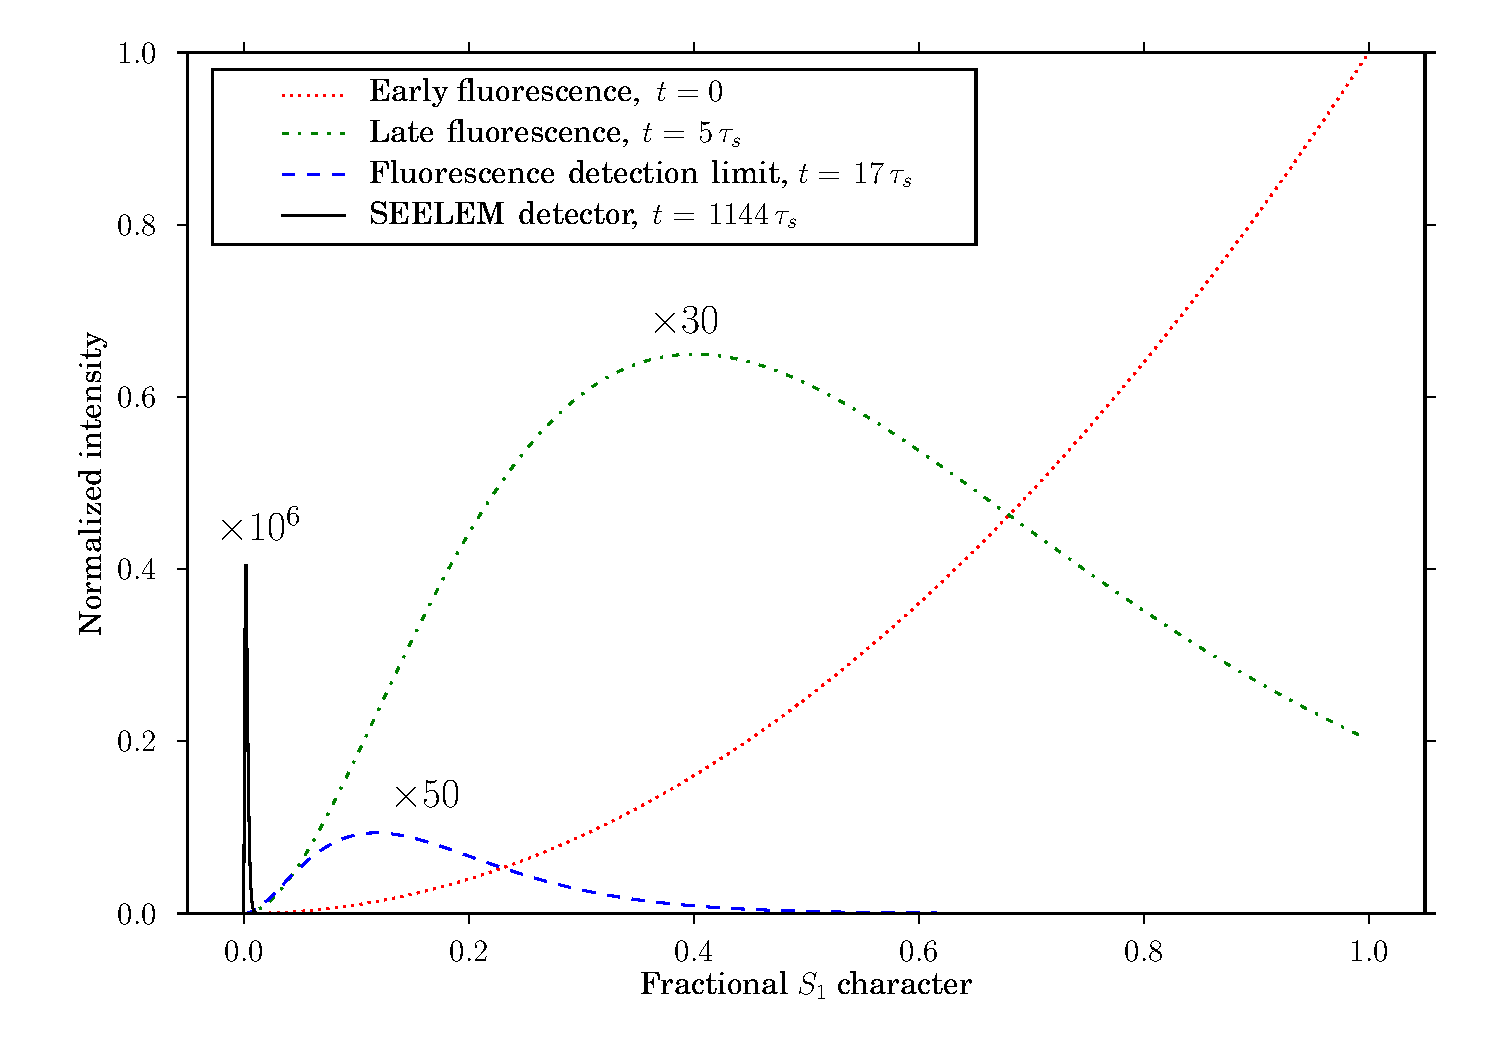
\includegraphics[width=7.5in,angle=90]{intensity-at-delay.pdf}
\end{figure}

Figure \ref{fig:int-at-rc} shows the dependence of fluorescence
intensity on fractional bright state character at several selectable
values of $R$.  At early fluorescence window times ($t \sim \tau_s$),
the fluorescence intensity is greatest for states with large amounts
of fractional bright state character ($2/R > 1$).  At a delay of $t =
R \tau_s = 5 \tau_s$, the fluorescence intensity equation
discriminates against states with large fractional bright state
character, since molecules in such states have already fluoresced with
high probability.  States with small fractional bright state character
are also discriminated against.  Molecules in such states have a low
probability of fluorescing in the time window under consideration.
The detectable fluorescence intensity may thus be ``tuned'' to a
chosen value of fractional bright state character merely by selecting
a time delay $R$, according to Equation \ref{eq:am-max}.

\POINT{Remove this paragraph?}  Note that the intensity expression
used here does not account for molecules moving out of the field of
view of the fluorescence detection optics.  We consider only the
distribution of bright state character \emph{among molecules that
  remain within the field of view at time $R$}.  However, since there
is no momentum transfer from the excitation photon to the molecule,
the rate of molecules exiting the field of view is independent of
bright state character.  Thus, the statistical properties of the
spectrum in the frequency domain, involving only fluorescence
intensity ratios between molecules with differing fractional bright
state character, are undistorted by molecules moving out of the field
of view.

\TODO{Move this to beginning.}  For the $S_1$ electronic state of
acetylene, $\tau_s=270$ ns \cite{ochi91}.  The field-of-view of the
fluorescence detection optics is about 5 mm, which amounts to a
maximum viewing time of about 5 $\mu$s, about $18\tau_s$, for
molecules in the molecular beam, which has an average velocity of
$10^3$ m/s.  At times later than $10\tau_s$, no molecules remain
within the fluorescence field of view.  This places an upper limit on
the value of $R$ that can be selected in our fluorescence experiments.
Figure \ref{fig:int-at-rc} shows the intensity equation for the long
time limit of fluorescence detection, $18\tau_s$.

The SEELEM detector used in our experiments detects metastable
molecules after a 309 $\mu$s flight time.  If we set aside some
aspects of SEELEM detectivity and consider only its detection
sensitivity to bright state character, we arrive at the following
equation for SEELEM detection probability (Chapter 2, equation 28):
\begin{equation}
  \label{eq:seelem-prob-s}
  P_{SEELEM}^{(s)} \propto a_m^4 \; \exp \left( -R_c \, a_m^2 \right).
\end{equation}
(This is a good approximation to the overall detection sensitivity of
SEELEM, including electron ejection probability resulting from
fractional $T_3$ electronic character, in the weak coupling limit.)
The SEELEM detection probability equation above has the same
functional form as Equation \ref{eq:int-m}.  Thus, the SEELEM detector
may be viewed in this limited sense as an extreme discriminator for
detecting states with small fractional bright state character.

Acetylene molecules in our apparatus are detected after an average
flight time of 309 $\mu$s, yielding an $R_c$ value of $1144$ for the
SEELEM detector.  This corresponds to a maximum detection probability
for states with $0.17\%$ bright state character.

\subsection{Delayed fluorescence of a model system}

Our next step is to examine how the characteristics of a
fluorescence intensity distribution change as we increase the time delay
$R$.  We model the interaction between a bright state and an
ensemble of dark states by generalizing from a two-level system.
Consider a Hamiltonian with only one dark state.  Define the two mixed
states $\ket{m=1,2}$ as
\begin{equation}
  \begin{split}
    \ket{1} &=  (1 - \alpha^2)^{1/2} \ket{s} + \alpha \ket{t}\\
    \ket{2} &= -\alpha \ket{s} + (1 - \alpha^2)^{1/2} \ket{t}.
  \end{split}
\end{equation}
The fluorescence intensity of both states, relative to a pure bright
state, is
\begin{equation}
  \begin{split}
    I_1 &= \frac{(1 - \alpha^2)^2}{\tau_s} \; \exp 
          \left[
            - R \, (1 - \alpha^2)
          \right]\\
    I_2 &= \frac{\alpha^4}{\tau_s} \; \exp 
          \left[
            - R \, \alpha^2
          \right],
  \end{split}
\end{equation}
and the ratio of the fluorescence intensities changes with time,
$t=R\tau_s$, as
\begin{equation}
  I_{12} = I_1 / I_2 = 
  \left(
    \frac{(1 - \alpha^2)}{\alpha^2}
  \right)^2
  \exp
  \left[
    - R \, (1 - 2\alpha^2)
  \right].
\end{equation}  \TODO{Explain behavior of this equation.  Prefactor
  determines initial ratio.  Long time limit, always approaches zero.}

\TODO{Rwrite this -- frame center of gravity in terms of intensity
  ratios.  Explain center of gravity.}  The fluorescence intensity
ratio may be incorporated into an equation for the dependence of
average detected intensity on $R$,
\begin{equation}
  \label{eq:ratio}
  \braket{I_{LIF}} = 
  \frac{\Delta E_{12}}{2} \,
  \left(
    \frac{I_{12}-1}{I_{12}+1}
  \right).
\end{equation}
Figure \ref{fig:ratio} shows the dependence of the intensity-weighted
center-of-gravity on the intensity ratio $I_{12}$.

\begin{figure}
  \caption{Center of gravity as a function of the intensity ratio
    $I_1$:$I_2$ for a two-state system.  At $t=0$, the initial center
    of gravity is a function of the mixing amplitude $\alpha$.  The
    center of gravity then shifts with the changing intensity ratio as
    delay time is increased, arriving at a limiting value of $-\Delta
    E_{12}/2$.}
  \label{fig:ratio}
  \centering
  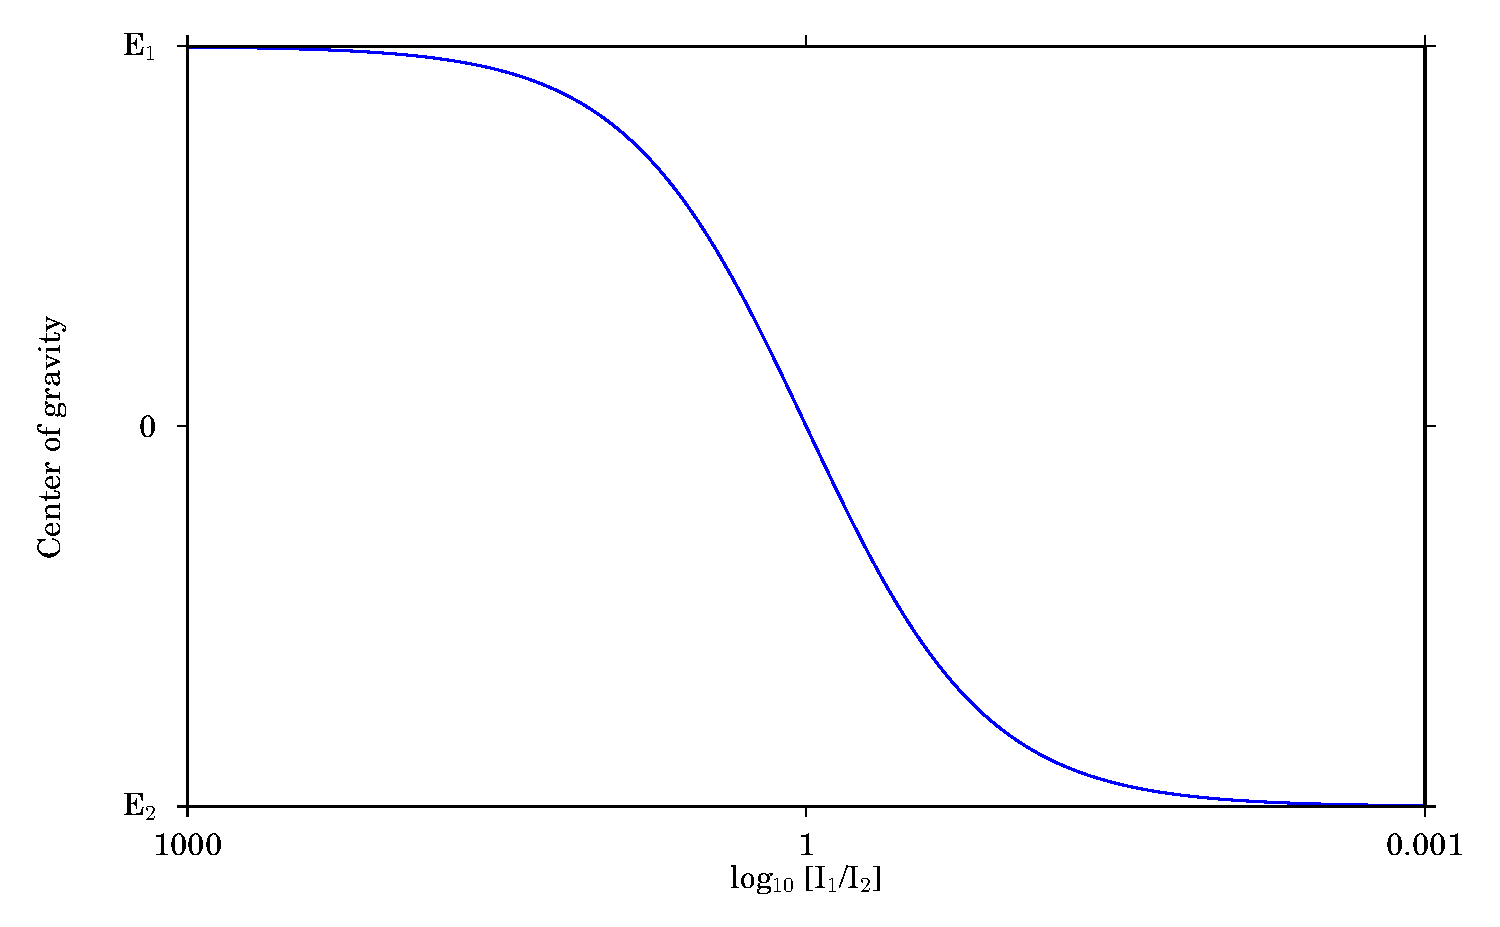
\includegraphics[width=6in]{cog-from-ratio.pdf}
\end{figure}

The initial intensity ratio at time $R_c=0$ is
\begin{equation}
  I_{12} = 
  \left(
    \frac{(1 - \alpha^2)}{\alpha^2}
  \right)^2.
\end{equation}
From this, the initial center of gravity can be found according to
Equation \ref{eq:ratio} or Figure \ref{fig:ratio}.  At large values of
$R_c$, the intensity ratio decreases to zero as $I_1 \ll I_2$, if the
states are not 50:50 mixed.  As the ratio decreases toward zero, the
intensity-weighted center of gravity approaches $-\Delta E_{12} / 2$.
The R-dependence of intensity ratios and the consequent shift in
center of gravity are shown in Figure \ref{fig:cog-devel}.  

\TODO{Say this more clearly.  Explain weak and strong limits.} One
interesting aspect of the center of gravity shift shown in Figure
\ref{fig:cog-devel} is the sudden onset of the shift at small mixing
coefficients.

\begin{figure}
  \caption{(Top) Time development of the intensity ratio for
    a two state system. (Bottom) Time development of the center of
    gravity for a two state system.}
  \label{fig:cog-devel}
  \centering
  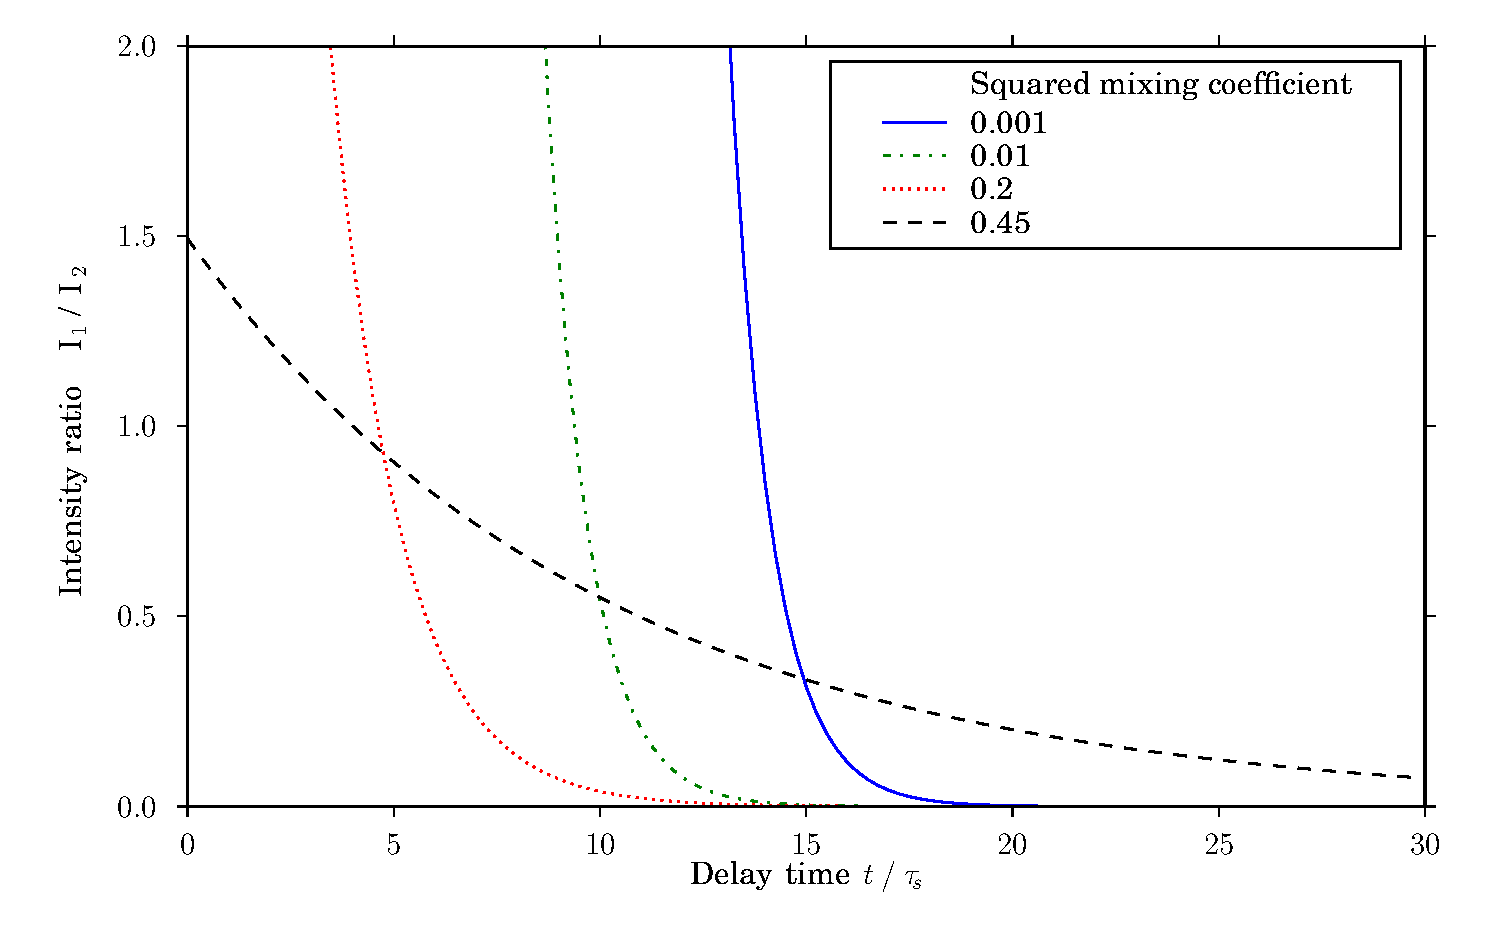
\includegraphics[width=6in]{ratio-development.pdf}
  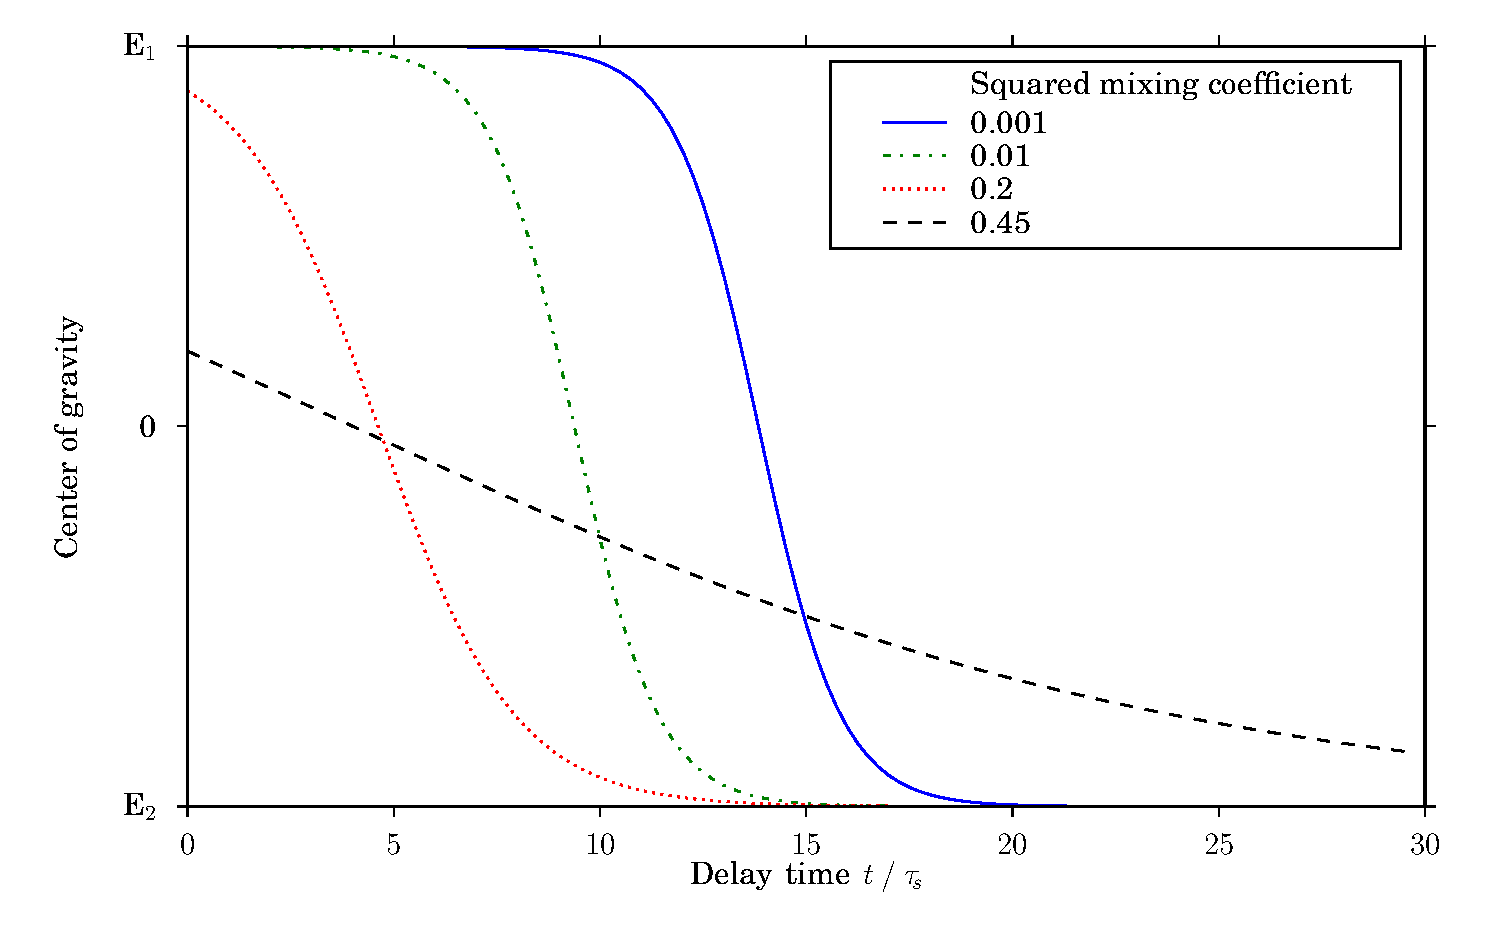
\includegraphics[width=6in]{cog-development.pdf}
\end{figure}

% \subsection{Delayed fluorescence of a series of rotational
%   transitions}

% Information about the relative energy of a doorway level can be
% recovered from the statistical properties of delayed fluorescence as a
% function of rotational quantum number.  \POINT{Continue explaining the
% general idea.}

% \POINT{Present energy level spacings.} For a near-symmetric prolate
% top in Hund's case ($b$), the spin-orbit selection rules are
% \cite{stevens73}
% \begin{equation}
%   \begin{split}
%     \Delta J &= 0 \\
%     \Delta N &= 0, \pm 1\\
%     \Delta K_a &= 0, \pm 1.
%   \end{split}
% \end{equation}
% \TODO{Rewrite this.}  Due to the $\Delta N$ selection rule, a singlet
% level $\ket{s;N=J}$ may interact with three rotational components of a
% dark triplet state: $F_1$, $\ket{\ell;N=J-1}$; $F_2$,
% $\ket{\ell;N=J}$; and $F_3$, $\ket{\ell;N=J+1}$.  The relative
% energies of the three components are, in terms of the singlet
% rotational quantum number $J$, \TODO{use different notation for
%   $\Delta B$?}
% \begin{equation}
%   \label{eq:components}
%   \Delta E_{s\ell}(J) = (E_{s} - E_{\ell}) +
%   \begin{cases}
%     \Delta B_{s\ell}J(J+1) + 2B_{\ell}J           
%     & F_1 \text{ component}\\
%     \Delta B_{s\ell}J(J+1)                      
%     & F_2 \text{ component}\\
%     \Delta B_{s\ell}J(J+1) - 2B_{\ell}J - 2B_{\ell} 
%     & F_3 \text{ component}.\\
%   \end{cases}
% \end{equation}
% In the approximation that $B_s \approx B_{\ell}$, the relative
% energies of the $F_{1,2,3}$ components change linearly when plotted
% against $J$.  The energy of the $F_2$ component relative to the
% singlet state has a slope of approximately zero, while the $F_1$ and
% $F_3$ components have slopes of approximately $\pm2B$.  The relative
% energy differences between $S_1$ and $T(F_1,F_2,F_3)$ are plotted in
% Figure \ref{fig:components}.

% \begin{figure}
%   \caption{\TODO{Change xlabel to $J$.}  Reduced term value plot of
%     the three singlet$\sim$triplet roational components permitted by
%     the spin-orbit operator in Hund's case ($b$).  The $F_1$ component
%     corresponds to...  }
%   \label{fig:components}
%   \centering
%   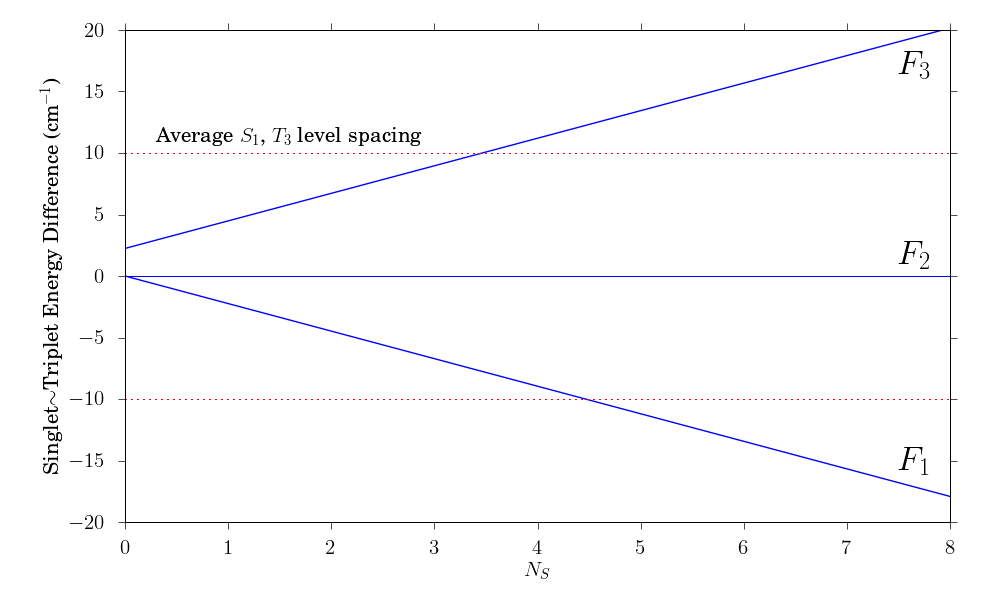
\includegraphics[width=6in]{f-components.png}
% \end{figure}

% Based on the existing assignment of a local $T_3$ perturber in $S_1$
% $3 \nu_3$ $K_a$=1, as well as $T_3$ geometries prediced by \emph{ab
%   initio} calculations, we expect the product $\Delta B_{s\ell}J(J+1)$
% to remain small compared to $2BJ$ for any combination of $S_1$ and
% $T_3$ vibrational levels \cite{mishra04, ventura03, thom07} up to the
% maximum $J$ values ($J<8$) observed in our experiment .  \POINT{The
%   figure is a good approximation to what we expect from the molecule.}

% The total first-order spin-orbit matrix element between two
% rovibrational states is given by the product of three factors: an
% electronic spin-orbit matrix element, a vibrational overlap factor,
% and a rotational factor arising from angular momentum coupling.  The
% rotational factors are given for the general case of polyatomic
% molecule asymmetric tops by Stevens and Brand \cite{stevens73}.  Plots
% of the spin-orbit rotational factors are presented in Figure
% \ref{fig:rotational-factors-0} for singlet levels with $K$=0, $K$=1
% (Figure \ref{fig:rotational-factors-1}), and $K$=2 (Figure
% \ref{fig:rotational-factors-2}).  With the exception of $\Delta N =
% \Delta K = 0$ interactions, the rotational factors quickly approach
% their asymptotic limits, usually between 0.1 and 0.6.  Even at low
% values of $J$, the variation of rotational factor with rotational
% quantum number is always less than a factor of 2.  \POINT{These
%   variations are trumped by energy denominator and vibrational overlap
%   effects.}

% \begin{figure}
%   \caption{Rotational factors for spin-orbit coupling in polyatomic
%     molecules, $K_s$=0}
%   \label{fig:rotational-factors-0}
%   \centering
%   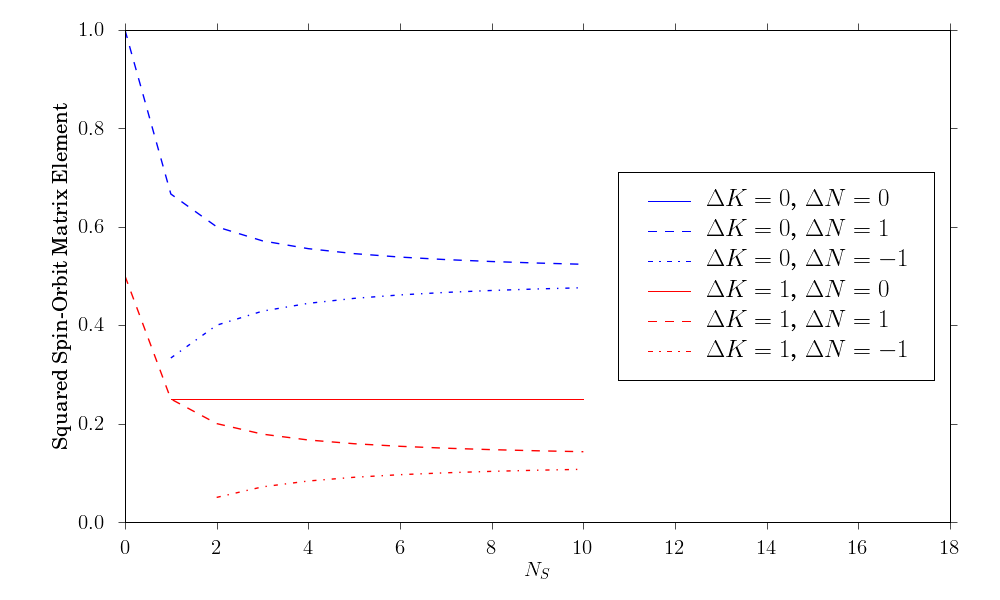
\includegraphics[width=6in]{rotational_factors_k0.png}
% \end{figure}

% \begin{figure}
%   \caption{Rotational factors for spin-orbit coupling in polyatomic
%     molecules, $K_s$=1}
%   \label{fig:rotational-factors-1}
%   \centering
%   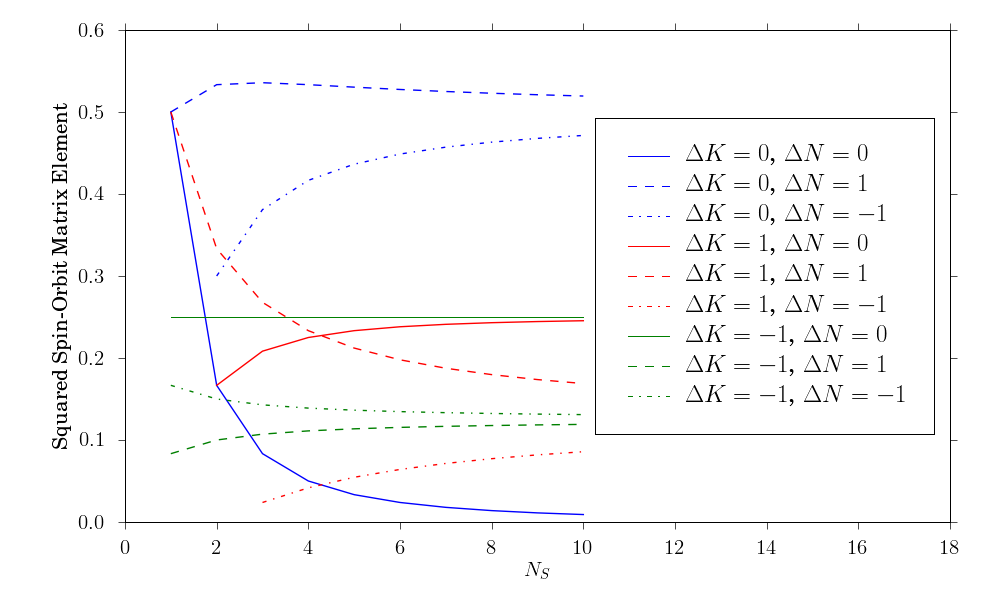
\includegraphics[width=6in]{rotational_factors_k1.png}
% \end{figure}

% \begin{figure}
%   \caption{Rotational factors for spin-orbit coupling in polyatomic
%     molecules, $K_s$=2}
%   \label{fig:rotational-factors-2}
%   \centering
%   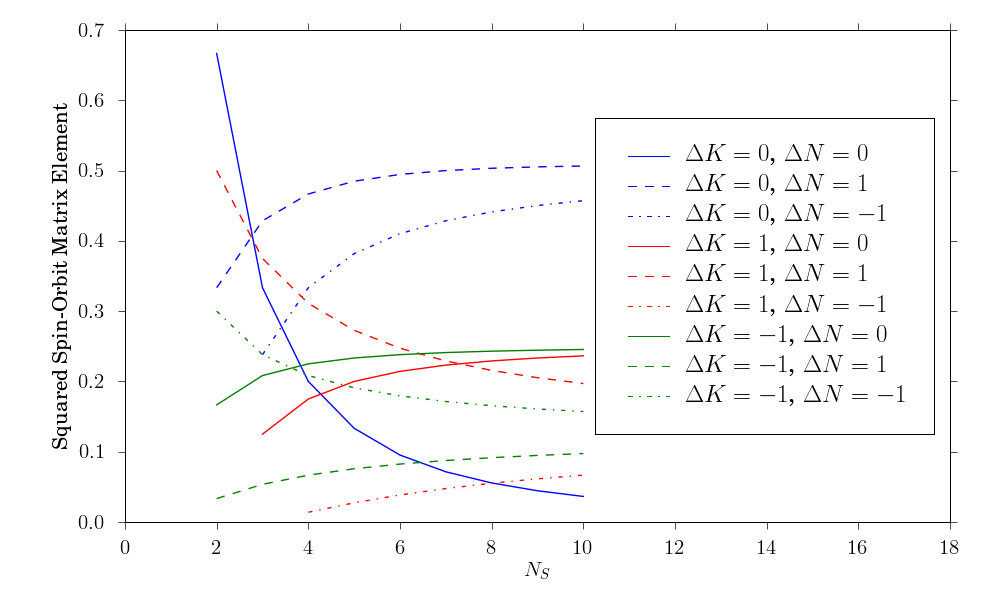
\includegraphics[width=6in]{rotational_factors_k2.png}
% \end{figure}

% \POINT{Expect vibrational factor to vary greatly.}  The effects of
% widely varying vibrational overlap factors divide $S_1 \sim T_3$
% perturbations into two classes: those where $H_{st}/\Delta E_{st} \ll
% 2B$, and those where $H_{st} / \Delta E_{st}$ is on the order of $2B$.

% \POINT{Explain pattern when $H_{st}/\Delta E_{st} \ll 2B$.}
% Perturbations in the first class, observable as a level shift, will
% occur only once in the spectrum.  However, once a triplet level with
% small vibrational overlap is found at a particular $J$, its energy
% above or below the perturbed singlet level may be found according to
% Equation \ref{eq:components}.

% \POINT{Explain pattern when $H_{st}/\Delta E_{st} \approx 2B$.}
% Perturbations falling into the second class will affect the
% singlet$\sim$triplet coupling at several values of $J$; these are the
% distant $T_3$ doorways with which we are most concerned.  \TODO{Plot
%   mixing coefficients of distant doorways as a fcn of rotational
%   quantum number.  Trend will be: weakly coupled states turn on/off
%   suddenly, strongly coupled states are visible for several values of
%   $N$.}





















% \section{Experiment}

% \TODO{Adapt this from paper.}  SEELEM is a versatile and sensitive
% technique for investigating molecules in ``dark'' (weakly-fluorescing)
% metastable states populated by laser excitation.1-6 In the SEELEM
% experiment, a molecular beam of acetylene is excited by a $\sim$5 ns
% FWHM pulsed tunable laser into spin-rotation-vibration eigenstates of
% metastable electronic states via weak, nominally forbidden
% transitions. After excitation, the long-lived species must travel 35
% cm before colliding with an Au metal detector surface, where an
% electron is ejected in a de-excitation process. Two criteria must be
% met for electron ejection by a metastable species. First, the vertical
% electronic energy of the metastable approaching the surface must
% exceed the work function of the metal ($\Phi_{\text{Au}}$ = 5.1
% eV). Second, the radiative lifetime of the detected metastable
% eigenstate ($\tau_\text{rad}$) must exceed the flight time from the
% point of laser excitation to the SEELEM surface ($\Delta$t=300
% $\mu$s).

% A sample of acetylene (BOC gases) at a backing pressure of one
% atmosphere was pulsed through a 0.5 mm diameter nozzle (Jordan Valve)
% operating at 10 Hz into a diffusion pumped vacuum chamber at
% $\sim$5\e{-5} torr.  An Nd:YAG pumped, frequency-doubled dye laser
% (220 nm) excited the acetylene molecules in the pulsed jet expansion 2
% cm downstream from the nozzle orifice.  \TODO{Include laser details
%   here.}

% UV-LIF was detected perpendicular to the plane defined by the
% intersection of the pulsed molecular and laser beams using f/1.2
% collection optics, a fluorescence filter (UG-11) to reduce scattered
% laser light, and a PMT (Hamamatsu model R375).  The time-varying
% UV-LIF signal was averaged on a digital oscilloscope (LeCroy \TODO{get
%   model}) at each laser frequency.  The resulting oscilloscope trace,
% containing 500 evenly spaced voltage levels over a 5 \microsec\
% timespan ($dt$ = 10 ns), was transferred to a PC for analysis.

% Simultaneous SEELEM detection was performed in a separate,
% differentially pumped vacuum chamber.  Following laser excitation,
% molecules in the pulsed expansion passed through a conical skimmer
% (3mm diameter), forming a collimated molecular beam in the SEELEM
% detection chamber.  The detector chamber was diffusion pumped (Varian
% 600) to maintain a pressure of $\sim$4\e{-7} torr during operation.
% The SEELEM detector surface, a 2.5 cm diameter region of heated
% (300\degrees\ C) Au foil, was located 35 cm downstream from the point
% of laser excitation.  The SEELEM detector was identical to that used
% in the previously described apparatus with Au foil ($\Phi_{\text{Au}}$
% = 5.1 eV) as the detector surface.

% Electron signals from the SEELEM detector were collected using pulse
% counting techniques.  Electrons ejected from the metal surface were
% detected by a nearby electron multiplier (ETP, SGE Instruments, Model
% 14831H).  The collection plate of the multiplier was biased at +100V
% to attract electrons.  The electron multiplier signal was sent to a
% discriminator (EG\&G/Ortec Model 9301), and then to a PC-operated
% multichannel scalar (Oxford Tennelec Nucleus Inc. MCS-II v2.091),
% where the total number of electrons was summed.  The typical signal
% level for SEELEM detection of acetylene was 2-20 counts per laser
% pulse.

% Both SEELEM and LIF signals were averaged over 100 laser shots at each
% laser frequency.  The frequency increment was typically
% $\sim$0.015 \rcm\ in the doubled output, although several detailed
% spectra were recorded with a 4$\times$ smaller step size.  





























% \section{LIF/SEELEM spectroscopy of four $S_1$ vibrational levels above
%   the $S_1 \sim T_3$ seam of intersection}

% %%%%%%%%%%%%%%%%%%%%%%%%%%%%%%%%%%%%%%%%%%%%%%%%%%%%%%
% %%
% %% INSERT LEVEL TABLE HERE
% %%
% %%%%%%%%%%%%%%%%%%%%%%%%%%%%%%%%%%%%%%%%%%%%%%%%%%%%%%

% \begin{table}[t]
%   \caption{The four acetylene $S_1$ vibrational levels considered in
%     this study, listed here, have total vibronic energies in the
%     critical region above the $S_1 \sim T_3$ electronic seam of
%     intersection ($\simeq 45300$ \rcm) and below the first
%     dissociation barrier ($\simeq 46300$ \rcm).  An order-of-magnitude
%     estimate of the observed SEELEM:LIF intensity ratio is included.}
%   \label{table:termvals}

%   \centering
%   \begin{tabular}{rlrr}
%     \\
%     Subband & & $T_0$ (\rcm ) & SEELEM:LIF\\
%     \midrule
%     $2^23^1$ \Ka{1} & $\leftarrow$ $0_0$ & 46009 & $10^{-2}$ \\
%     $3^24^2$ \Ka{1} & $\leftarrow$ $0_0$ & 45812 & $10^{-1}$ \\
%     $2^13^2$ \Ka{1} & $\leftarrow$ $0_0$ & 45677 & $10^{-1}$ \\
%       $3^3$ \Ka{2} & $\leftarrow$ $4_1$ & 45352 & 1 \\
%   \end{tabular}
% \end{table}

% %%%%%%%%%%%%%%%%%%%%%%%%%%%%%%%%%%%%%%%%%%%%%%%%%%%%%%
% %%
% %% END OF LEVEL TABLE
% %%
% %%%%%%%%%%%%%%%%%%%%%%%%%%%%%%%%%%%%%%%%%%%%%%%%%%%%%%


% The choice of $S_1$ vibrational levels in this study was guided by two
% considerations: the energetic accessibility of $T_3$ vibrational
% levels and absence of predissociation effects.  The $S_1 \sim T_3$
% electronic seam of intersection, located near $3^3$ \Ka{1}, $T_0
% \simeq 45300$ \rcm, provides a lower energy bound for the
% accessibility of $T_3$ levels from the $S_1$ electronic surface.
% \TODO{Citations.}  Above the seam of intersection, any $S_1$ level
% may, in principle, have a large vibrational overlap with one or more
% $T_3$ levels.  The first dissociation barrier, located near $3^4$
% \Ka{1}, $T_0 \simeq 46300$ \rcm, provides an upper energy bound for
% this study.  \TODO{Citations.}  Below this barrier, predissociation
% pathways are not energetically accessible, and do not complicate the
% study of $S_1 \sim T_3$ interactions.

% We consider four $S_1$ sublevels in this energy region, appearing in
% the $\tilde{A}^1A_u \leftarrow \tilde{X} ^1\Sigma_g^+$ spectrum of
% acetylene.  The levels are listed with their total (rotationless)
% vibronic energy, $T_0$, in Table \ref{table:termvals}.  Included in
% the table is an order-of-magnitude estimate of the SEELEM:LIF
% intensity ratio observed in the spectrum.  To determine this quantity,
% relative LIF intensties were estimated from a low resolution jet
% spectrum reported by Merer and coworkers \cite{merer03}.  The absolute
% SEELEM intensity was then divided by the estimated LIF intensity, and
% normalized to the largest SEELEM:LIF ratio.

% We observe that the highest energy state in our study has the lowest
% SEELEM:LIF intensity ratio.  Rather than total energy, the SEELEM:LIF
% intensity ratio is determined by the number of quanta in mode 3.  This
% observation is in agreement with previous estimations of SEELEM:LIF
% intensity ratios in acetylene \astate\ \cite{humphrey97}, and with
% measurements of the Zeeman anticrossing density \cite{dupre91}.

% We observe no systematic splittings at adjacent rotational levels in
% any of the spectra, which would indicate the presence of a local $T_3$
% doorway level, as in $3^3$ \Ka{1}.  Evidence of energetically distant
% $T_3$ doorway levels is found, however, in both the SEELEM and LIF
% spectra of these sublevels.  To characterize the spectral signatures
% of energetically distant doorway levels, we discuss the SEELEM/LIF
% spectrum of each sublevel individually.


% \subsection{The $3^24^2$ \Ka{1} sublevel: evidence of an
%   energetically distant $T_3$ doorway level plus a localized $T_3$
%   level crossing}

% % Spectrum: Dec05n 2006, p.86 of 9/2006--1/2007 notebook.

% %%%%%%%%%%%%%%%%%%%%%%%%%%%%%%%%%%%%%%%%%%%%%%%%%%%%%%
% %%
% %% INSERT 3^2 4^2 FIGURES HERE
% %%
% %%%%%%%%%%%%%%%%%%%%%%%%%%%%%%%%%%%%%%%%%%%%%%%%%%%%%%


% \begin{figure}
%   \caption{Simultaneously recorded SEELEM (upper trace) and LIF (lower
%     trace) spectra of the $3^24^2$ \Ka{1} sublevel of the \astate\
%     state of \ce{C2H2}.  The LIF spectrum is integrated in two time
%     regions: an early time window ($0.5\tau_s-2\tau_s$, solid trace)
%     and a delayed time window ($10\tau_s-18\tau_s$, dashed trace).
%     The peak positions are blueshifted in the delayed fluorescence
%     spectrum for all transitions, with the exception of Q(2).
%     Perturbations from a level of slightly lower energy are apparent
%     in the delayed fluorescence spectrum of the Q(2) and R(1)
%     transitions.}
%   \label{fig:spectrum-32b2}
%   \centering
%   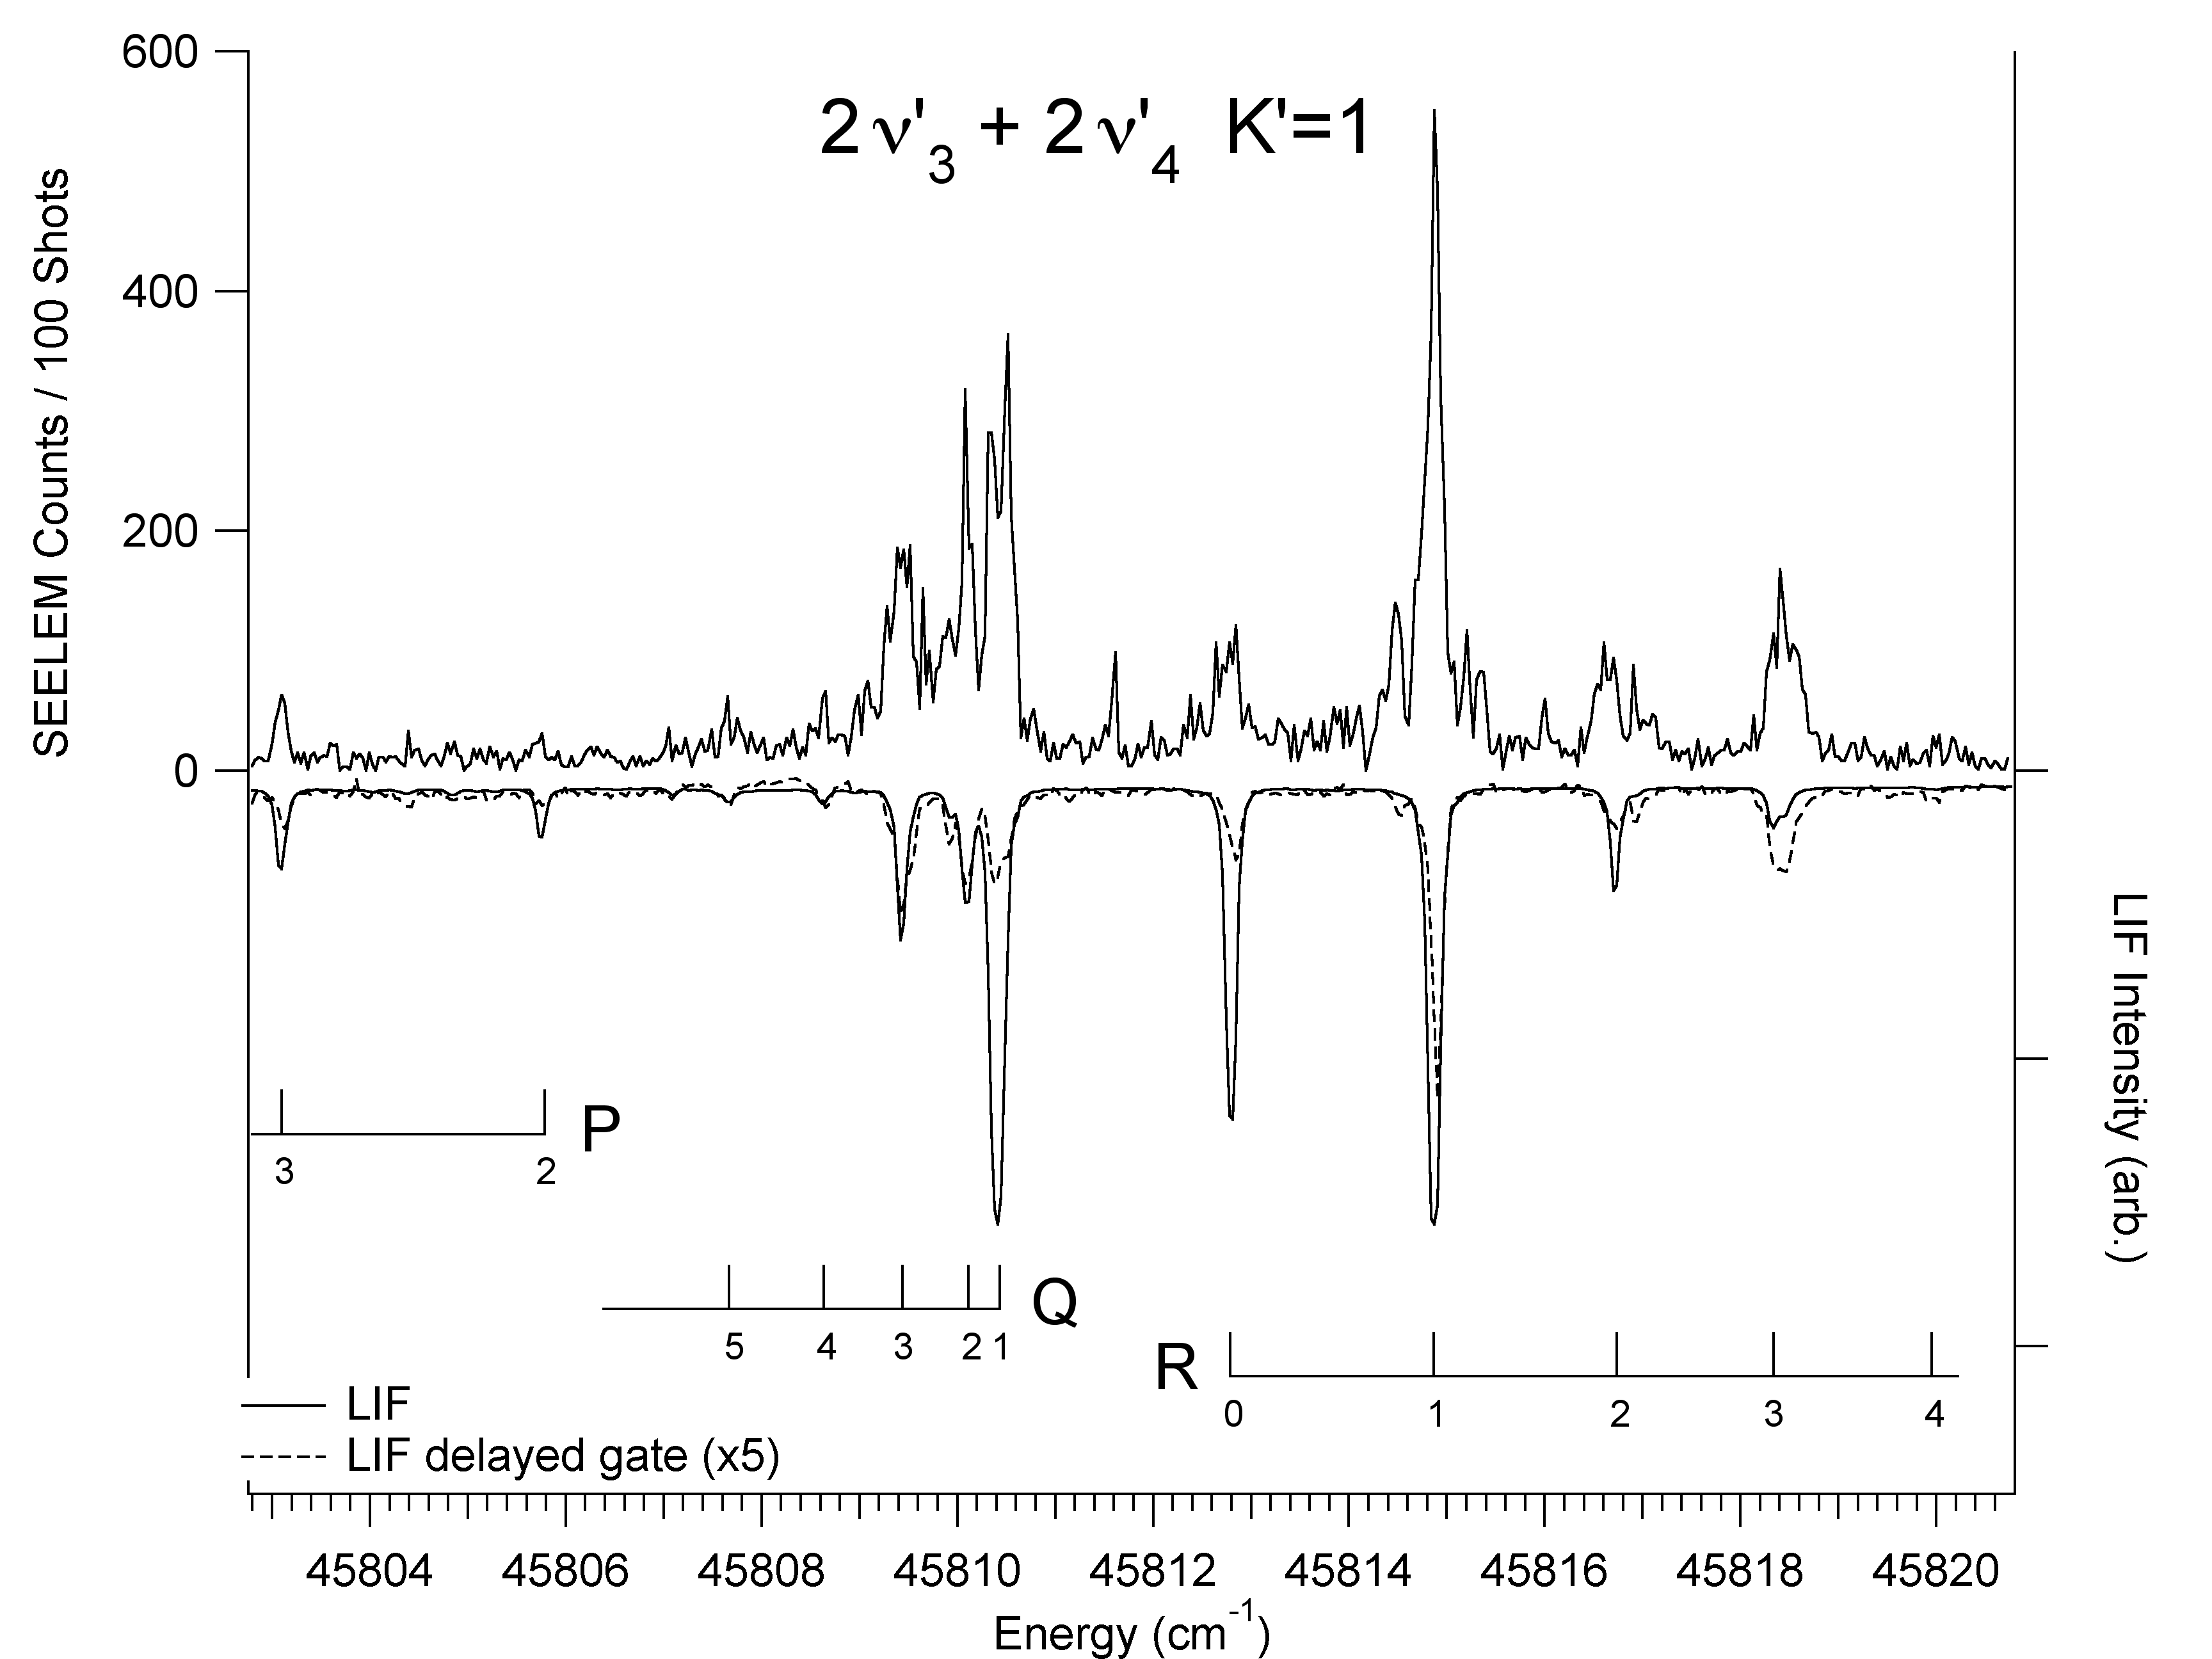
\includegraphics[width=7in,angle=90]{acetylene-32b2-p3r4.png}
% \end{figure}

% \begin{figure}
%   \caption{Dependence of the intensity-weighted center of gravity on
%     delay for a series of individually resolved transitions, Q(1$-$3)
%     (top), and R(0$-$3) (bottom), in the LIF spectrum of $3^24^2$
%     \Ka{1}.  Perturbations in the Q(2) and R(1) transitions cause the
%     center of gravity to deviate from that of the other transitions as
%     the delay time is increased.}
%   \label{fig:32b2-cog-delay}
%   \centering
%   \vspace{5mm}
%   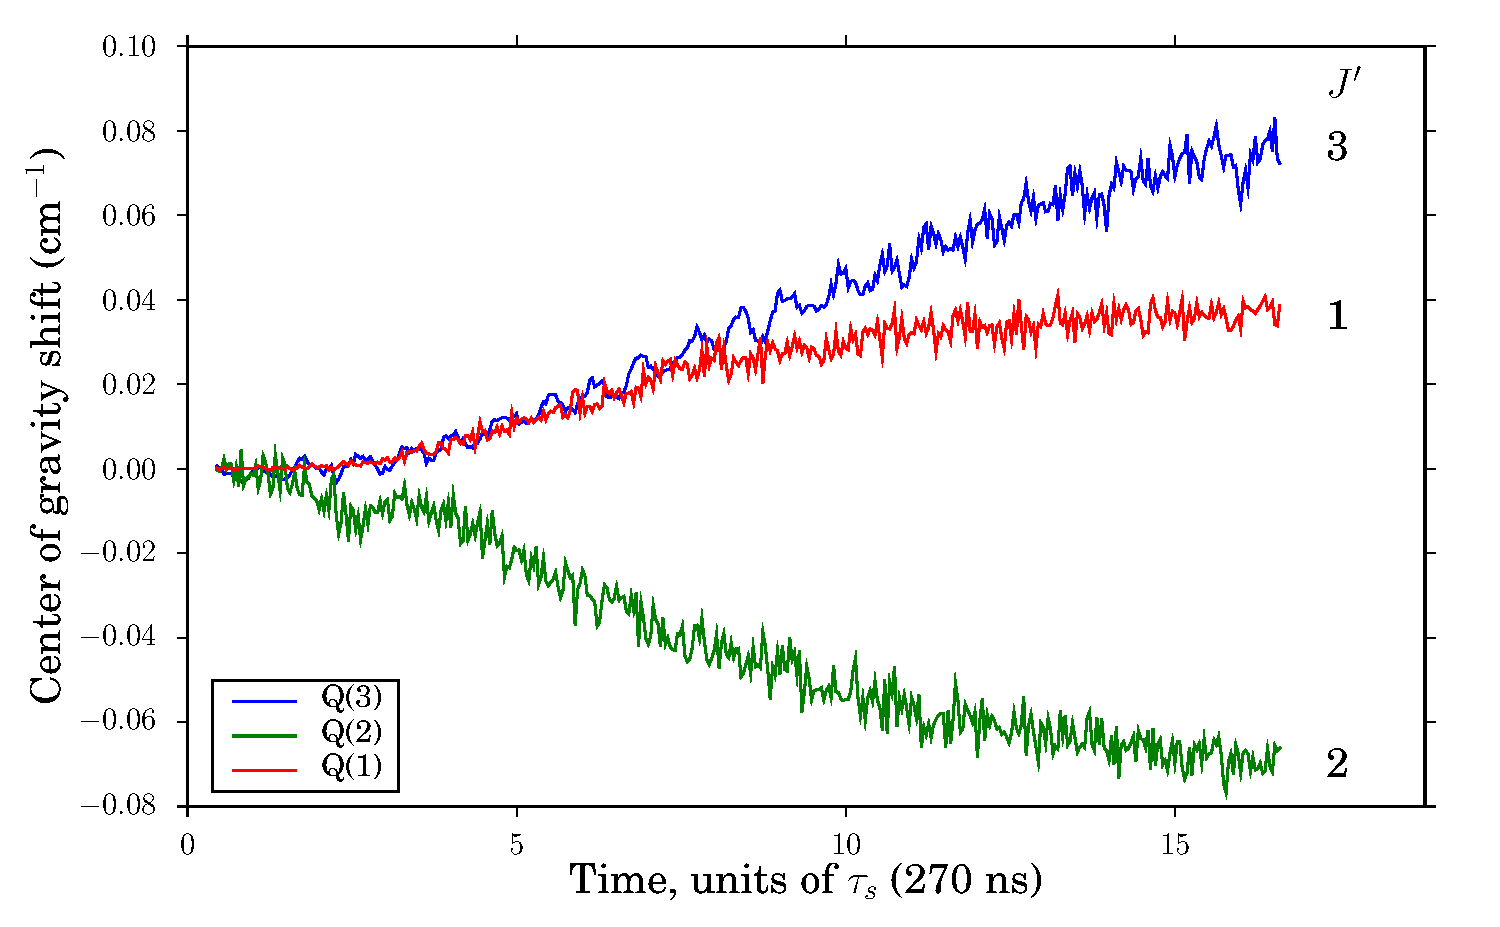
\includegraphics[width=6in]{32b2-q123-cog-delay.pdf}
%   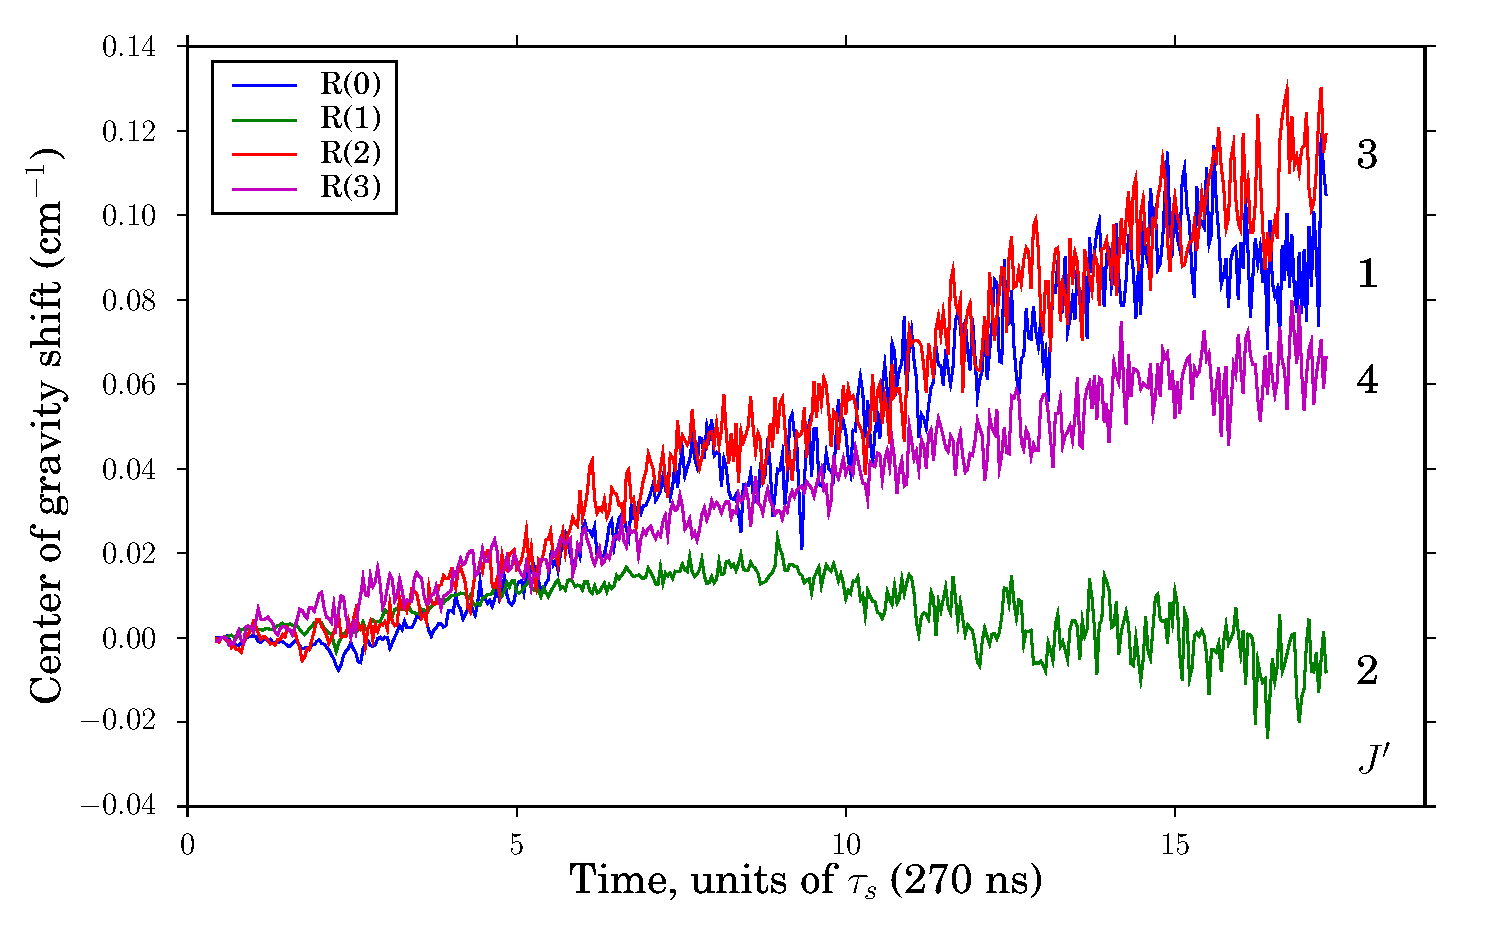
\includegraphics[width=6in]{32b2-r0123-cog-delay.pdf}
% \end{figure}


% %%%%%%%%%%%%%%%%%%%%%%%%%%%%%%%%%%%%%%%%%%%%%%%%%%%%%%
% %%
% %% END OF 3^2 4^2 FIGURES
% %%
% %%%%%%%%%%%%%%%%%%%%%%%%%%%%%%%%%%%%%%%%%%%%%%%%%%%%%%

% The $3^24^2$ level is the upper member of the $3^2B^2$ polyad of the
% acetylene \astate state, where $B = (4, 6)$.  The $\nu_4$ and $\nu_6$
% vibrations are strongly mixed by a-type Coriols and Darling-Dennison
% anharmonic resonances.  As a result, the nominal $3^24^2$ level
% contains essentially a 50:50 mixture of mode 4 and mode 6 basis
% character.  \TODO{Cite AHS.}

% The simultaneously recorded SEELEM/LIF spectrum of the $3^24^2$ \Ka{1}
% $\leftarrow$ $0_0$ subband of the \AtoX\ electronic spectrum is shown
% in Figure \ref{fig:spectrum-32b2}. To highlight the dependence of the LIF
% spectrum on delay time, two integration regions are used.  An early
% LIF fluorescence spectrum is generated by gating the fluorescence signal between $0.5\tau_s$ and $2\tau_s$.
% A second, delayed LIF spectrum is generated from integration in the time window $10\tau_s-18\tau_s$.  The peak poisition of several transitions is
% clearly blueshifted in the delayed LIF spectrum relative to the early
% LIF.  Peak offsets in the R(0), R(1), and R(4) transitions are
% approximately 0.08 \rcm.

% The intensity envelopes in the delayed LIF spectrum closely resemble
% those in the SEELEM spectrum.  As we established in the preceeding
% section, the SEELEM spectrum appears as the the long-time-delay limit
% of the LIF spectrum, in the absence of a local level crossing with a
% $T_3$ doorway level.

% To more closely examine the dependence of the LIF spectrum on time
% delay, the intensity-weighted center of gravity (Formula (from last
% section)) is plotted for each transition as a function of delay time.
% The plot for Q-branch transitions was generated from another dataset,
% not shown here, recorded at approximately $4 \times$ smaller energy
% intervals, resulting in increased signal to noise.  With the exception
% of the R(1) and Q(2) transitions, the center of gravity increases by
% 0.04-0.12 \rcm\ over the delay range $0.5\tau_s-18\tau_s$.  Such a
% consistent increase in delayed center of gravity with delay time
% indicates the presence of a non-local $T_3$ doorway level that is
% higher in energy, according to Formula (from preceeding section).

% % The interaction is observed in both parities of the singlet at
% % $J'=1$ and $3$.  A doorway level with $K_T=0$ would The doorway
% % level cannot be assigned as $K_T=0$.  \emph{e}/\emph{f} symmetry
% % selection rules the interaction is present in both parities of the
% % singlet, .  Two possibilities remain for $K_T$

% A perturbation is present in the LIF spectrum of two transitions, Q(2)
% and R(1).  The relative intensity of the perturbations in the delayed
% fluorescence is stronger than that of the main comonent of the
% transition, indicating that they arise from levels with longer
% zero-order fluorescence lifetimes than the singlet.  Indeed, the R(1)
% perturbation is observable only in the delayed LIF spectrum, where a
% relative intensity increase causes it to emerge from the wing of the
% main line.  The perturbation in the R(1) transition, having upper
% state quantum number $J'=2$, is located at an energy of -0.33 \rcm\
% below the main component at 45814.87 \rcm.  The perturbation in Q(2),
% also having $J'=2$, is located at an energy of -0.17 \rcm\ relative to
% the peak of the strong, nominally singlet LIF transition at 45810.08
% \rcm.  

% The presence of two local perturbations at the same $J'$, arising from
% levels with a long zero-order lifetime, and not appearing in
% transitions with adjacent values of $J'$, can be explained by the
% presence of a level crossing involving the $F_1$ or $F_3$ component of
% a $T_3$ level having a small matrix element.  According to Formula
% (from last section), the relative energy of a $T_3$ level in this case
% is $\pm 2B \simeq \pm 2$ \rcm\ at $J'=1$ and $3$.  At $J'=2$, the singlet
% and triplet perturber are not 50:50 mixed, thus the matrix element
% must be appreciably smaller than half the energy separation.  This
% places an upper bound in the matrix elements of about $0.01$ \rcm.  At
% $J'=1$ or $3$, the increase in energy denominator from 0.2 \rcm\ to 2
% \rcm\ would make the perturabtion $100$ times weaker, precluding its
% observation in LIF.

% A lone SEELEM peak is observed in the band gap at 45811.6 \rcm,
% approximately 2 \rcm\ above the Q(3) transition at 45809.5 \rcm.  It
% is possible that this peak arises from the same weakly perturbing
% $T_3$ level.  Unfortunately, this position is overlapped with another
% transition in the R-branch, so it is impossible to check the other
% parity in this spectrum.  However, if we assign the transition in the
% band gap as $J'=3$, it must also be assigned as the $F_3$ component of
% the triplet level, $N_T=J'+1=4$, in order to be located at $+2$ \rcm\
% instead of $-2$ \rcm.  As a consequence, the triplet level must have a
% rotationless vibronic energy of $45811 - 6B \simeq 45804$ \rcm.

% We have examined a singlet sublevel, $3^24^2$ \Ka{1}, which shows
% evidence of interaction with an energetically distant $T_3$ doorway to
% higher energy.  A perturbation with small matrix element was observed
% at $J'=2$, and an assignment of $\Delta N=+1$ was suggested based on
% the observation of a weak transition in the SEELEM spectrum.  The
% assignment of $N_T$ determines that the energy of the perturbing
% triplet level is $-6$ \rcm\ relative to the singlet. If the assignment
% is not made, the perturbing level may also be located at an energy of
% $+4$ \rcm\ relative to the singlet.

% Local, weak perturbations from $T_3$ levels are common in the spectra
% of \astate\ acetylene, as we will see in the following examples.  In
% cases where $N_T$ or $K_T$ can be assigned, the relative energy of
% weak, locally perturbing levels can be pinpointed.  In cases where
% $N_T$ or $K_T$ can be assigned for energetically distant $T_3$ doorway
% levels (levels with large matrix elements), the relative rotationless
% energy is determined to be either positive or negative.  This can then
% be checked against the dependence of intensity-weighted LIF center of
% gravity on time delay.

% \subsection{The $2^13^2$ \Ka{1} sublevel: assignment of $K_a$ for an
%   energetically distant $T_3$ doorway level}

% % Spectrum: Jan 16A+B, p.124--127 of 9/2006--1/2007 notebook, also
% % assignments on p.2 of 1/2007--3/2007 notebook.

% %%%%%%%%%%%%%%%%%%%%%%%%%%%%%%%%%%%%%%%%%%%%%%%%%%%%%%
% %%
% %% INSERT 2^1 3^2 FIGURES HERE
% %%
% %%%%%%%%%%%%%%%%%%%%%%%%%%%%%%%%%%%%%%%%%%%%%%%%%%%%%%

% \begin{figure}
%   \caption{Simultaneously recorded SEELEM (upper trace) and LIF (lower
%     trace) spectra of the $2^13^2$ \Ka{1} sublevel of the \astate\
%     state of \ce{C2H2}.  The LIF spectrum is integrated in two time
%     regions: an early time window ($0.5\tau_s-2\tau_s$, solid trace)
%     and a delayed time window ($10\tau_s-18\tau_s$, dashed trace).
%     The Q(1) and Q(2) transitions are redshifted in the delayed
%     fluorescence spectrum, in contrast to the Q(3,4,5,6) transitions.
%     The P(2) transition, having the same $J'$ but opposite parity from
%     Q(1), shows a similar redshift in the delayed fluorescence
%     spectrum.}
%   \label{fig:spectrum-2132}
%   \centering
%   \vspace{1cm}
%   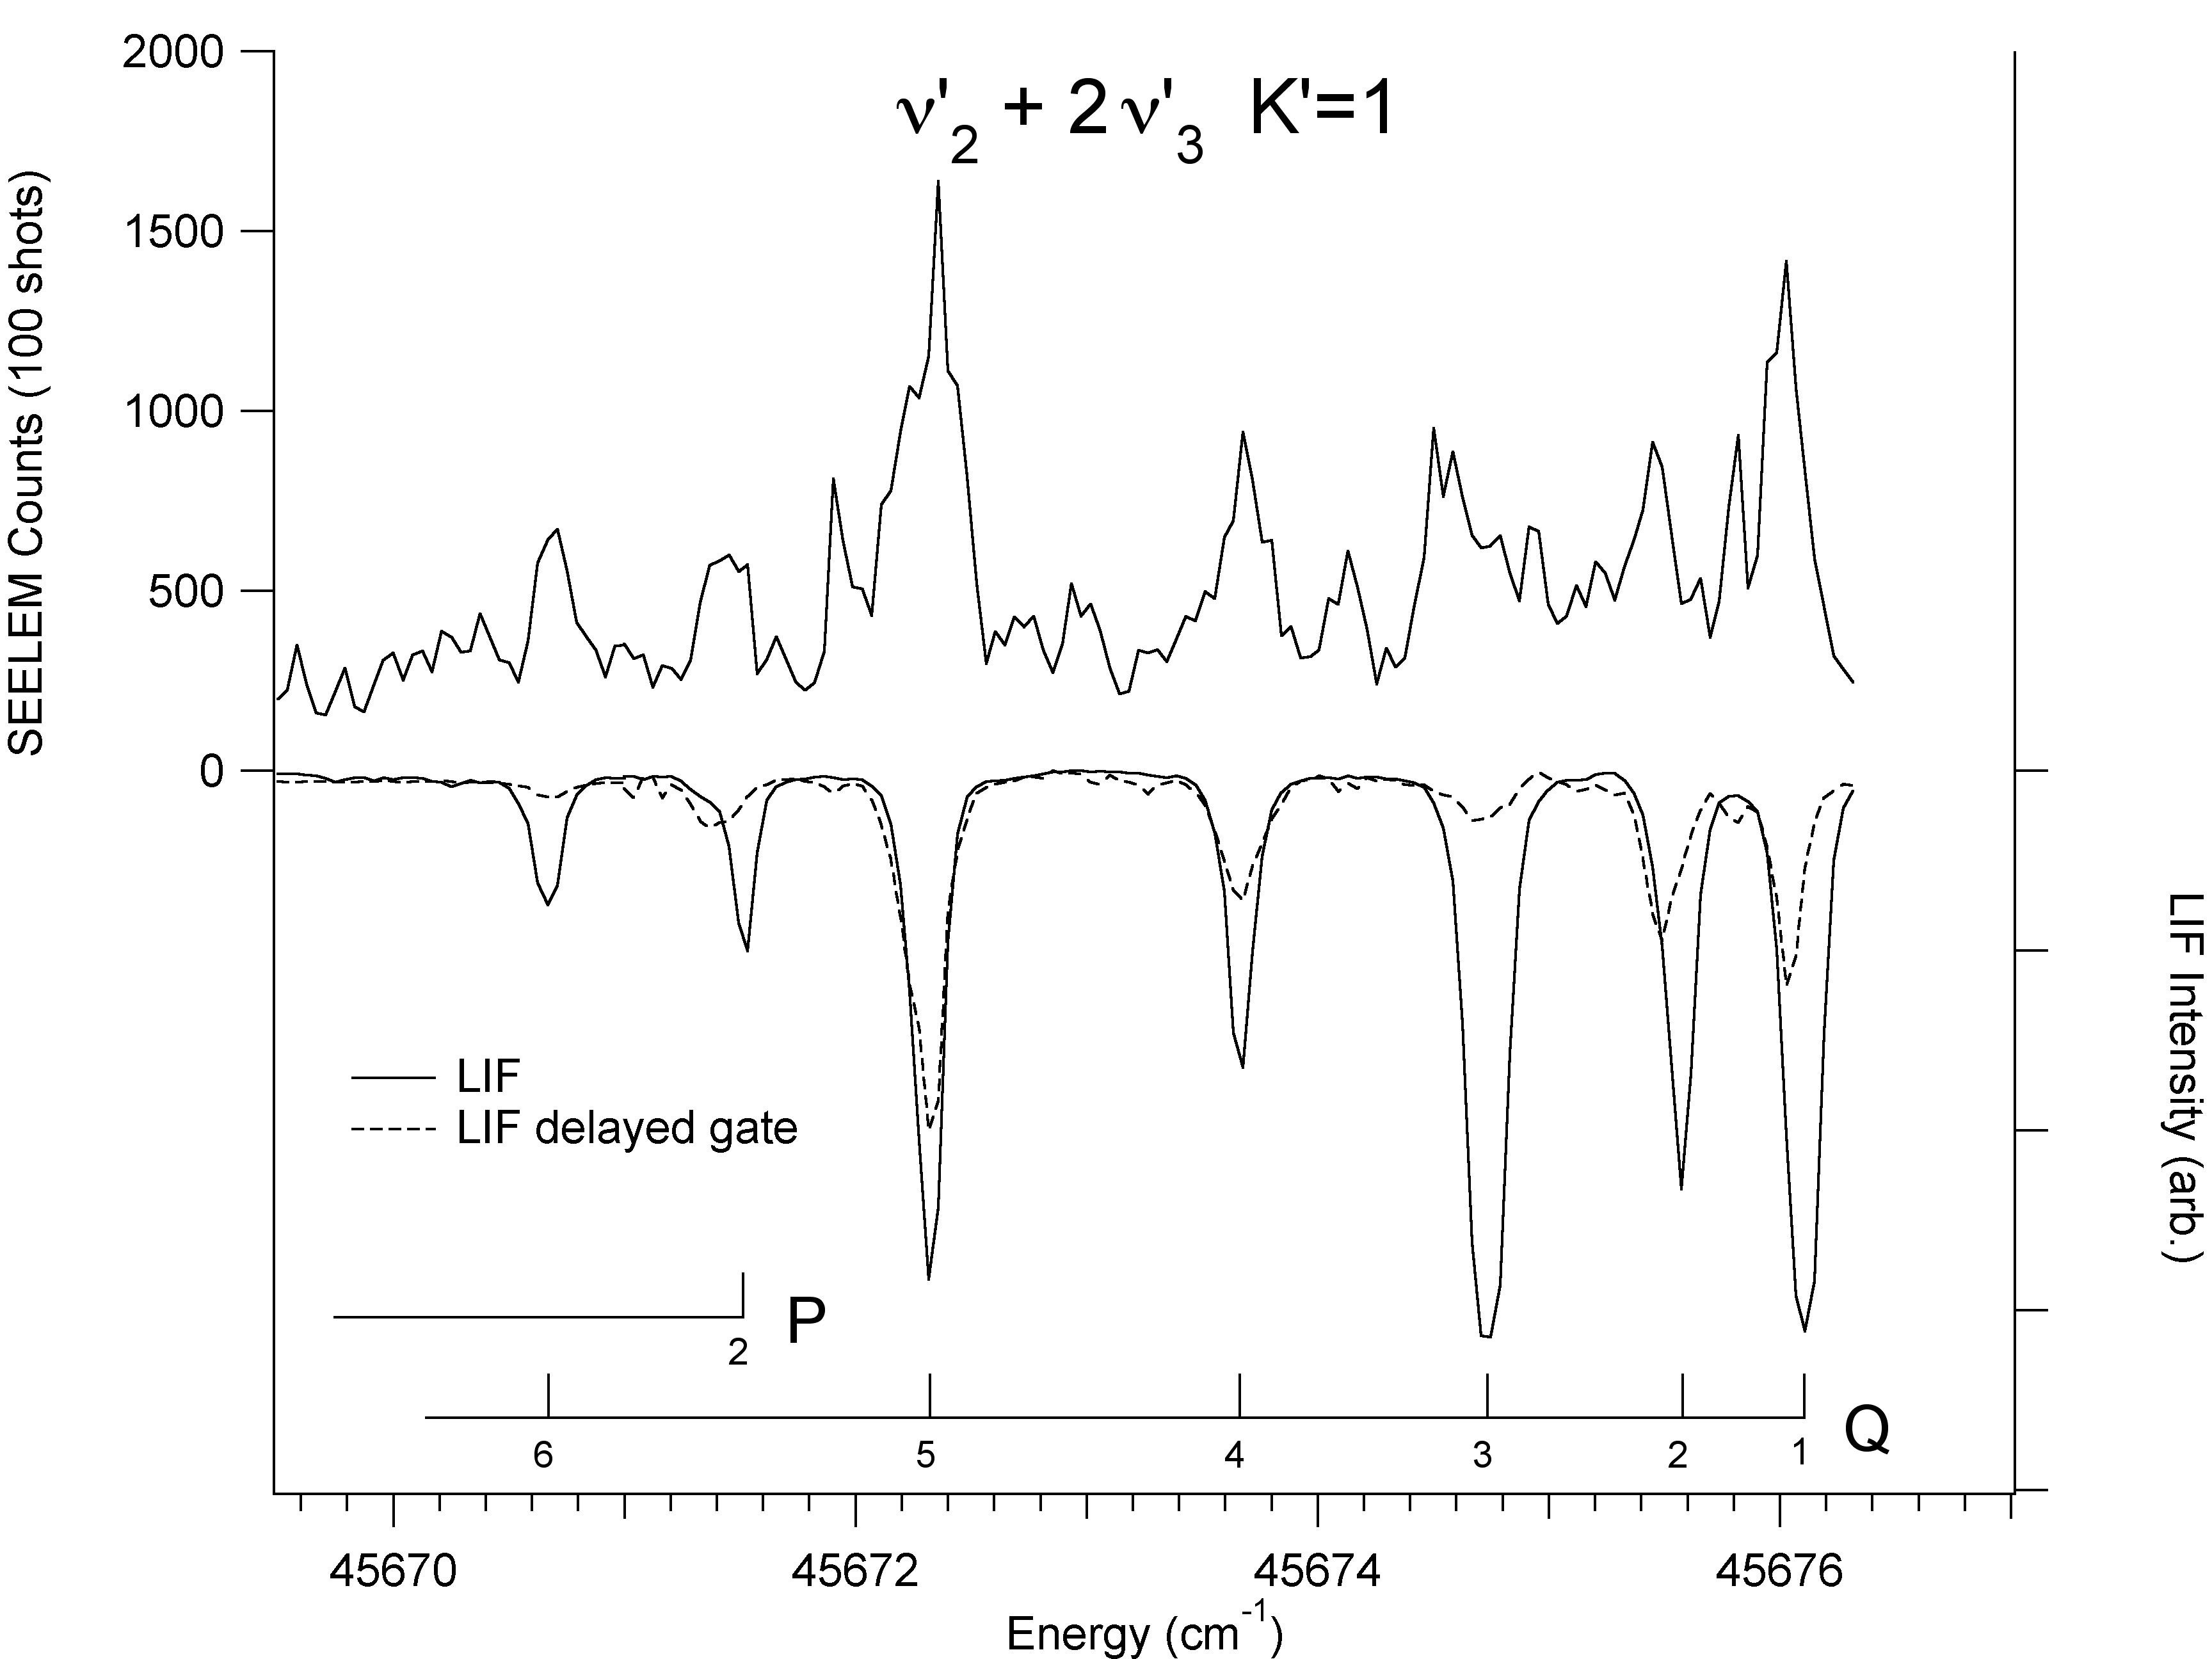
\includegraphics[width=7in,angle=90]{acetylene-2132-q6q1.png}
% \end{figure}

% \begin{figure}
%   \caption{Dependence of the intensity-weighted center of gravity on
%     delay for a series of individually resolved transitions, Q(1$-$5),
%     in the LIF spectrum of $2^13^2$ \Ka{1}.  The Q(1) and Q(2)
%     transitions arrive at peak positions identical to the those in the
%     SEELEM spectrum by a delay of $15\tau_s$.}
%   \label{fig:2132-q123456-cog-delay}
%   \centering
%   \vspace{1cm}
%   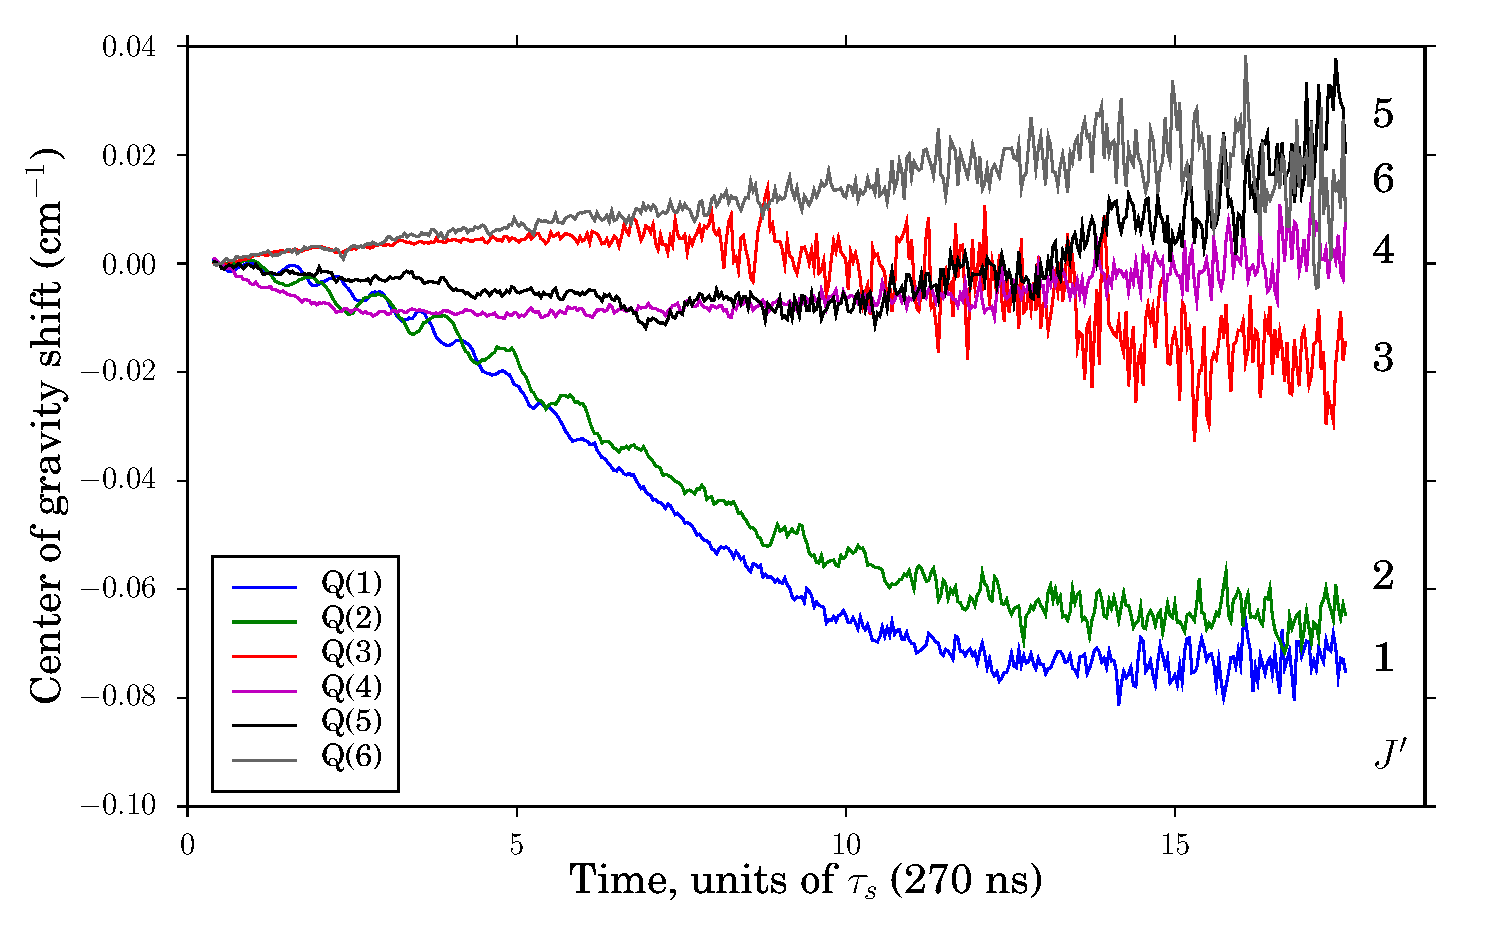
\includegraphics[width=6in]{2132-q123456-cog-delay.pdf}
% \end{figure}

% %%%%%%%%%%%%%%%%%%%%%%%%%%%%%%%%%%%%%%%%%%%%%%%%%%%%%%
% %%
% %% END OF 2^1 3^2 FIGURES
% %%
% %%%%%%%%%%%%%%%%%%%%%%%%%%%%%%%%%%%%%%%%%%%%%%%%%%%%%%

% We turn next to a sublevel containing an identical number of quanta in
% mode 3, $2^13^2$ \Ka{1}.  The overall SEELEM:LIF intensity ratio
% observed in the spectrum of this sublevel is similar to that of
% $3^24^2$ \Ka{1}, indicating a similar overall mixing angle with $T_3$
% doorway levels.

% The SEELEM/LIF spectrum of $2^13^2$ \Ka{1} $\leftarrow$ $0_0$ is shown
% in Figure \ref{fig:spectrum-2132}.  The LIF spectrum is integrated in
% early and delayed regions, using the same time limits as before.  The
% spectrum contains six Q-branch transitions (upper states of
% \emph{f}-symmetry, $J'=1-6$) and one P-branch transition (upper
% state of \emph{e}-symmetry, $J'=1$).  The delayed LIF peak position is
% redshifted by -0.08 \rcm\ relative to the early LIF peak position for
% two transitions ending in \emph{f}-symmetry states, Q(1) and Q(2).
% The sole \emph{e}-symmetry state observed in the spectrum, via the
% P(2) transition, is also redshifted in the delayed fluorescence
% spectrum by -0.12 \rcm.  The remaining transitions, Q(3,4,5,6), have
% the same peak position in the early and delayed LIF spectra.

% The dependence of the intensity-weighted center of gravity for all
% transitions in the Q-branch is shown in Figure
% \ref{fig:2132-q123456-cog-delay}.  The center of gravity for the Q(1)
% and Q(2) transitions changes by approximately -0.07 \rcm\ at a time
% delay of $15\tau_s$, in accord with the observation of changing peak
% position in the delayed LIF spectrum.  The center of gravity for the
% Q(3,4,5,6) transitions does not deviate by more than 0.02 \rcm\ from
% the initial position.

% We came to the conclusion in the preceding section that a consistent
% shift in center of gravity with delay indicates the presence of an
% energetically distant $T_3$ doorway level.  It seems paradoxical that,
% in this case, such an interaction would abruptly cease to occur at
% $J'=3$.  However, this behavior can be explained by the presence of a
% \emph{second} $T_3$ doorway level, located at higher energy than the
% singlet level.  An interaction with a second $T_3$ doorway level could
% cause the delayed center of gravity to be drawn higher in energy for
% the Q(3,4,5,6) transitions, if the interaction were to \emph{begin} at
% $J'=3$.

% Not only is such an interaction possible, but it leads to an
% assignment of $K_T$ for the second doorway level.  The selection rule
% $\Delta K = 0, \pm 1$ gives the possibilities of $K_T=$0, 1, and 2.  A
% level with $K_T=2$ has rotational levels beginning with $N_T=2$.  An
% $S_1 \sim T_3$ interaction with the $F_1$ components of such a level
% follows the selection rule $\Delta N = -1$, and would begin at
% $J'=N_S=3$, as observed in the spectrum.  All other combinations of
% $\Delta K$ and $\Delta N$ lead to $S_1 \sim T_3$ interactions
% beginning at $J'=1$ or $2$.  Thus, we can make the assignment of
% $K_T=2$ for the second $T_3$ doorway level.

% For the $F_1$ component of a triplet level, the relative
% singlet-triplet energy has a negative slope with respect to $J'$.  At
% $J'=3$, where the interaction with the second doorway level begins,
% the $F_1$ component is $6B \simeq 6$ \rcm\ lower in energy than the
% $F_2$ component.  As $J'$ increases, the relative energy of the $F_1$
% component decreases by $2B$ per $J'$.  Since the interaction must
% occur through an $F_1$ component in order to turn on at $J'=3$, and
% since the $F_1$ component is appreciably lower in relative energy than
% the other two components, we must conclude from the assignment of
% $K_T$ that the second $T_3$ doorway level is higher in energy than the
% singlet level.  This is, in fact, what is observed in the dependence
% of intensity-weighted center of gravity on delay time.

% The assignment of $K_T=2$ for the second doorway has further
% consequences.  The $K_T=2$ doorway level, higher in energy than the
% singlet level, must be accompanied by a $K_T=1$ doorway level at lower
% energy.  The energy separation between $K=1$ and $2$ sublevels of the
% same vibration is $3A_T$, where $A_T$ is the a-axis rotational
% constant for the triplet level in question.  According to \emph{ab
%   initio} calculations, the $A_T$ rotational constants for $T_3$
% vibrational levels vary between 10 and 30 \rcm \cite{thom07}.  This
% places the $K_T=1$ sublevel 30$-$90 \rcm\ lower in energy than the
% second doorway.

% Furthermore, the vibrational overlap factors for the two sublevels are
% identical, and the relative spin-orbit matrix elements are determined
% only by rotational factors.  Using formulas given by Stevens and
% Brand, the $K_T=1$ sublevel of the same vibration as the second
% doorway will have matrix elements about 5 times larger than those of
% the $K_t=2$ sublevel \cite{stevens73}.  Thus, the assignment of
% $K_T=2$ for the second doorway \emph{guarantees} the existence of
% another $5 \times$ stronger doorway level within a reasonable energy
% range below the singlet level.  Barring the existence of a
% \emph{third} strong doorway between the $K_a=1$ and $2$ sublevels of
% the second doorway vibration, we conclude that the first doorway is
% the $K_T=1$ sublevel of the same vibration.

% The analysis of LIF spectra at varying time delay has led to the
% detemination of relative energy and the $K$-assignment of two
% energetically distant $T_3$ doorway sublevels in the $2^13^2$ \Ka{1}
% $\leftarrow$ $0_0$ spectrum of acetylene \astate.  Such a conclusion
% is further supported by the appearance of the SEELEM spectrum of this
% vibronic transition, which shows striking similarity to the delayed
% fluorescence spectrum.  Peak positions in the delayed fluorescence
% spectrum are matched in SEELEM, even outside the main lines, for
% instance at 45675.9 \rcm\ and 45671.9 \rcm.  Agreement between the
% SEELEM spectrum and delayed fluorescence spectrum is evidence for a
% lack of $S_1 \sim T_3$ interference effects, which would manifest in a
% level crossing between the singlet level and a $T_3$ doorway
% \cite{altunata01}.


% \subsection{The $2^23^1$ \Ka{1} sublevel: a localized $T_3$
%   perturbation in the presence of small $S_1 \sim T_3$ matrix
%   elements}

% % Spectrum: Nov06d, see ``similitude'' calculations, p.62 of Sep
% % 2006--Jan 2007 notebook.

% %%%%%%%%%%%%%%%%%%%%%%%%%%%%%%%%%%%%%%%%%%%%%%%%%%%%%%
% %%
% %% INSERT 2^2 3^1 FIGURES HERE
% %%
% %%%%%%%%%%%%%%%%%%%%%%%%%%%%%%%%%%%%%%%%%%%%%%%%%%%%%%

% \begin{figure}
%   \caption{Simultaneously recorded SEELEM (upper trace) and LIF (lower
%     trace) spectra of the $2^23^1$ \Ka{1} sublevel of the \astate\
%     state of \ce{C2H2}.  The LIF spectrum is integrated in two time
%     regions: an early time window ($0.5\tau_s-2\tau_s$, solid trace)
%     and a delayed time window ($8\tau_s-12\tau_s$, dashed trace).  The
%     Q(1) and R(0) transitions, which have the same upper state quantum
%     number $J'=1$ but different parities, are shifted to opposite
%     directions in the delayed fluorescence spectrum.}
%   \label{fig:spectrum-2231}
%   \centering
%   \vspace{1cm}
%   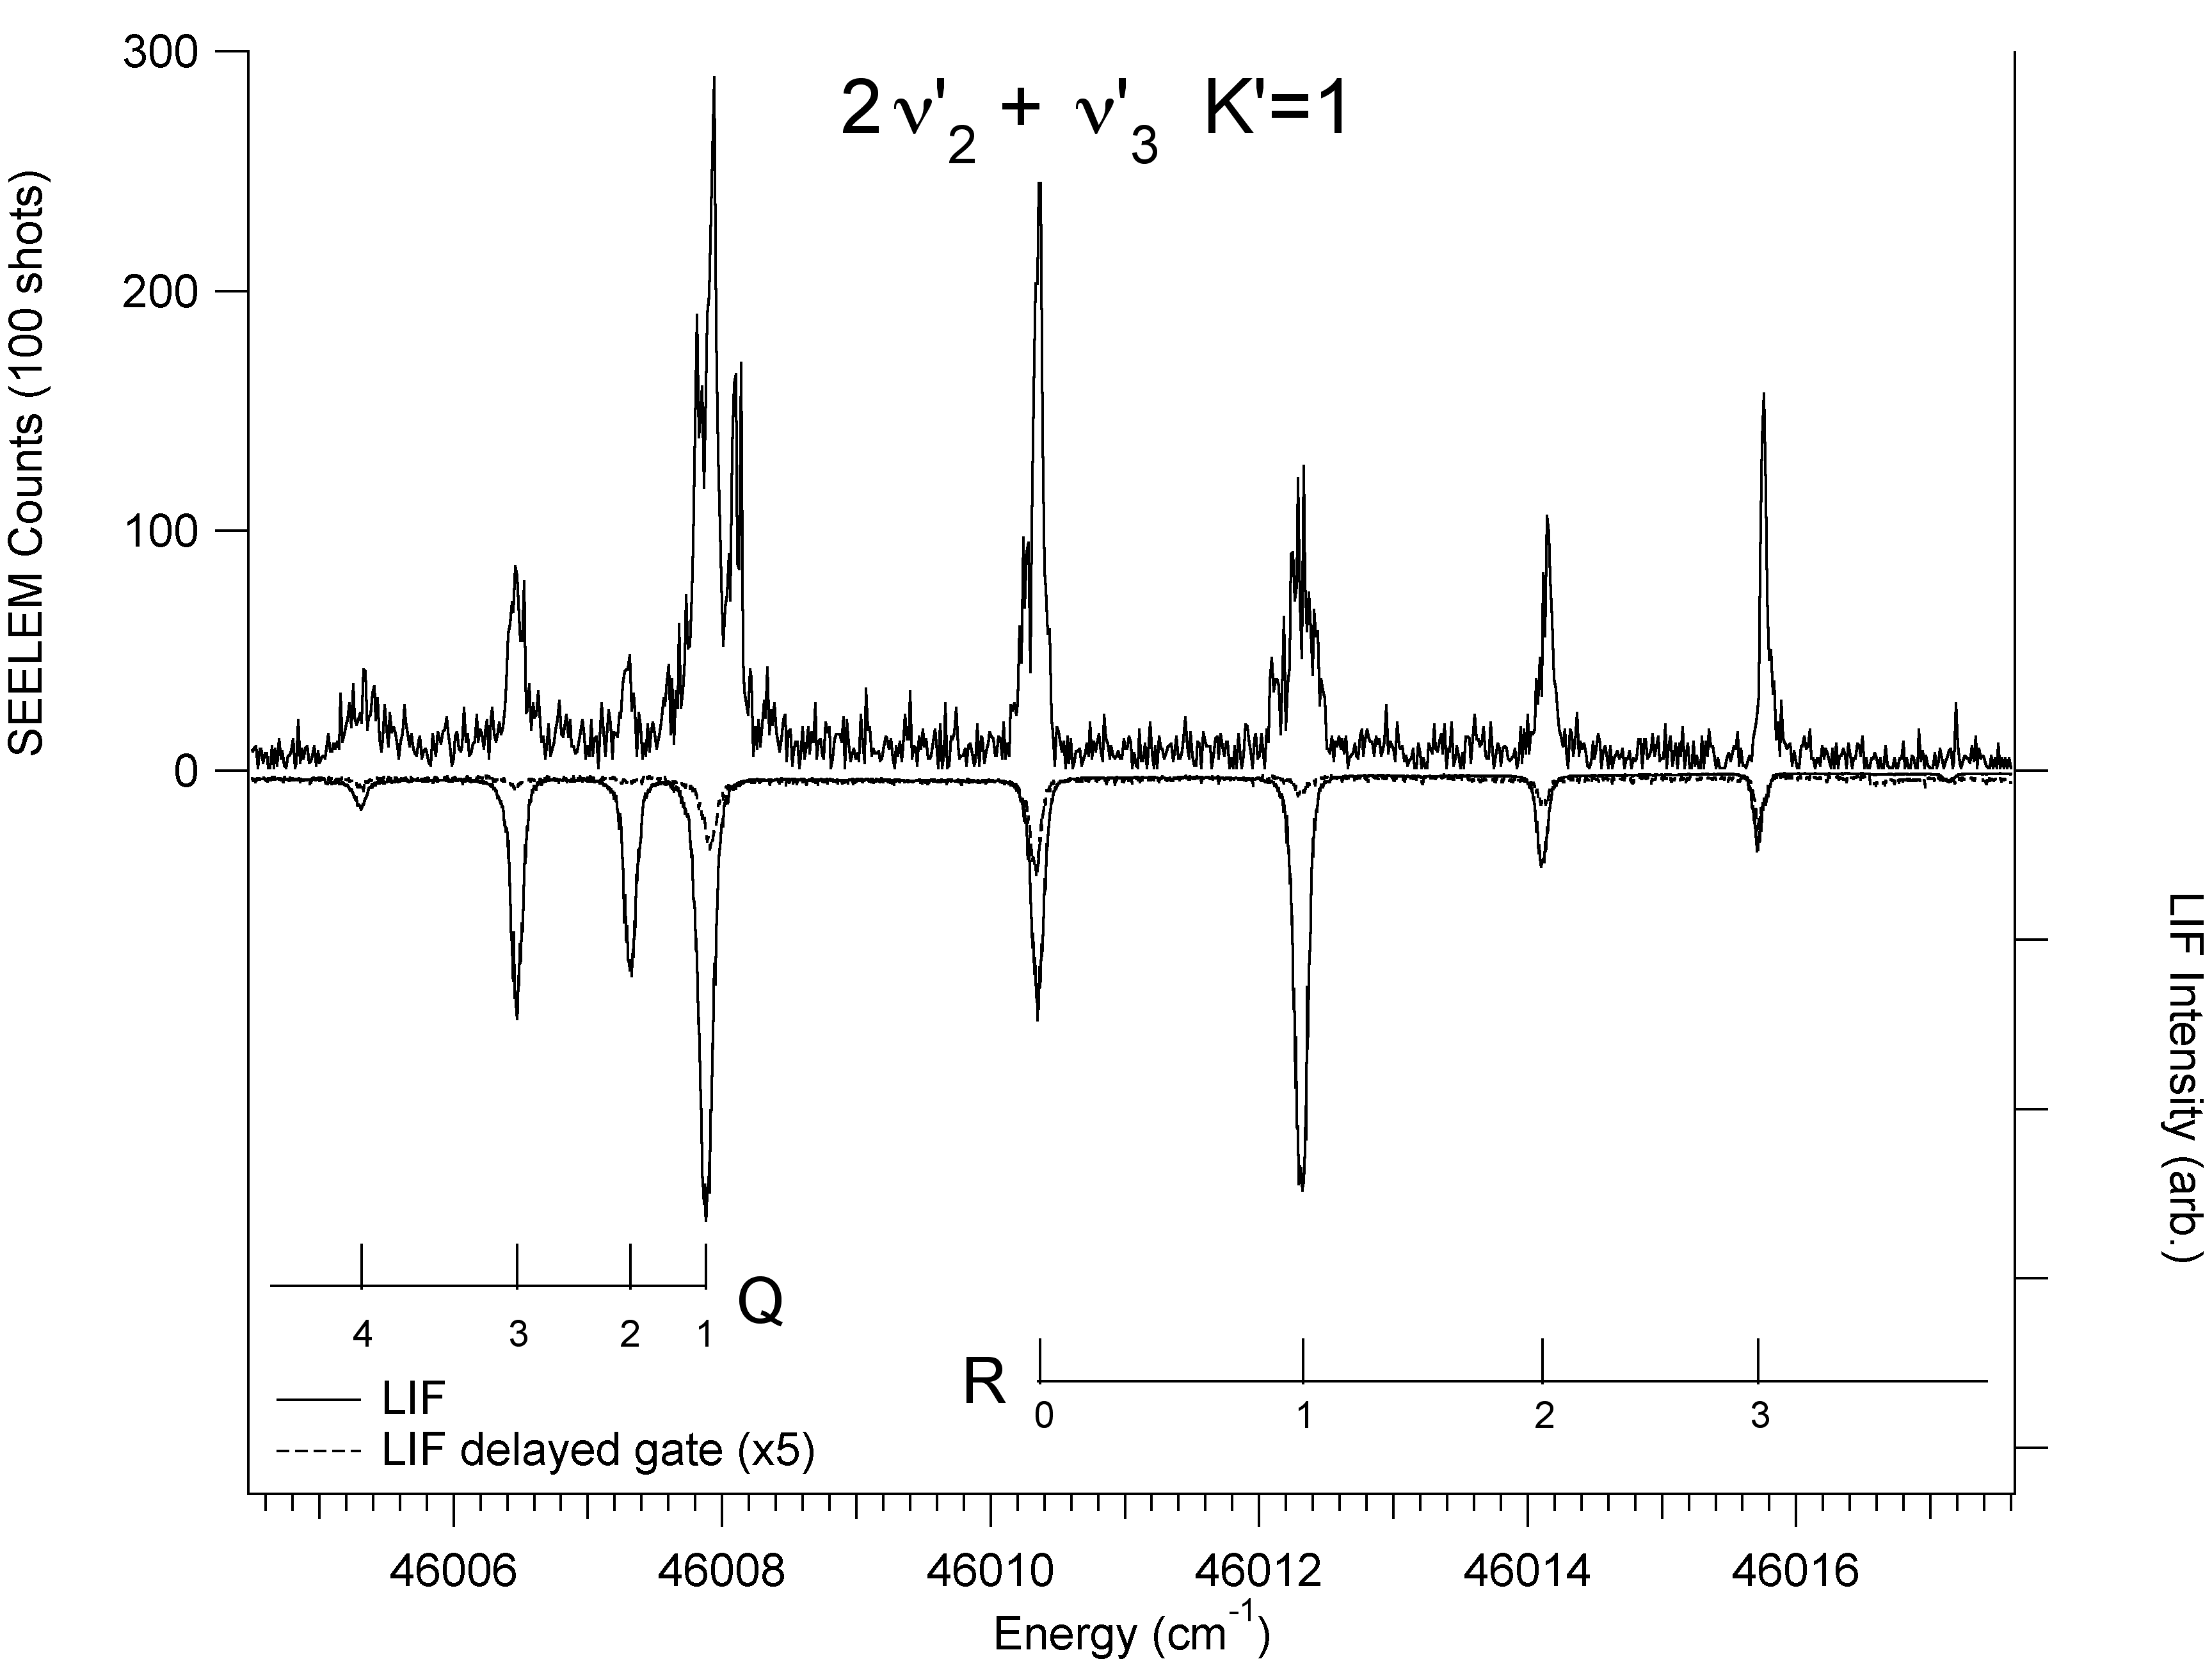
\includegraphics[width=7in,angle=90]{acetylene-2231-q4r3.png}
% \end{figure}

% \begin{figure}
%   \caption{Dependence of the intensity-weighted center of gravity on
%     delay for a series of individually resolved transitions, Q(1$-$4)
%     (top), and R(0$-$3) (bottom), in the LIF spectrum of $2^23^1$
%     \Ka{1}.  The center of gravity for the Q(1) transition rapidly
%     increases to its final value, where it matches the peak of the
%     SEELEM distribution at 46007.87$+$0.03 \rcm.  For the R(0)
%     transition, the center of gravity decreases at a nearly linear
%     rate to 46010.35$-$0.3 \rcm.}
%   \label{fig:2231-cog-delay}
%   \centering
%   \vspace{5mm}
%   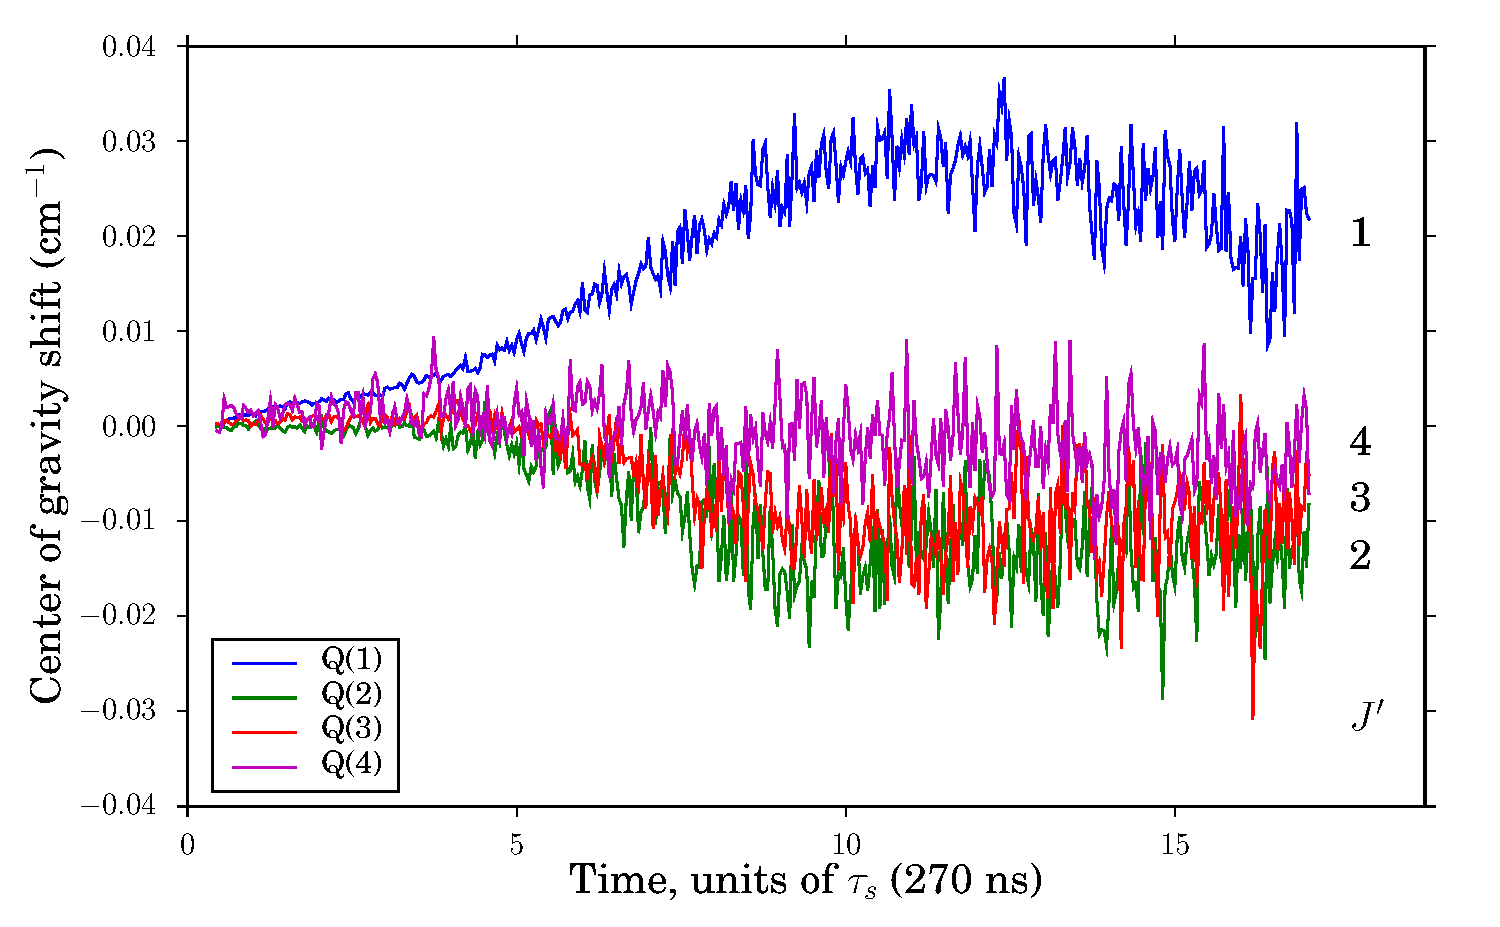
\includegraphics[width=6in]{2231-q1234-cog-delay.pdf}
%   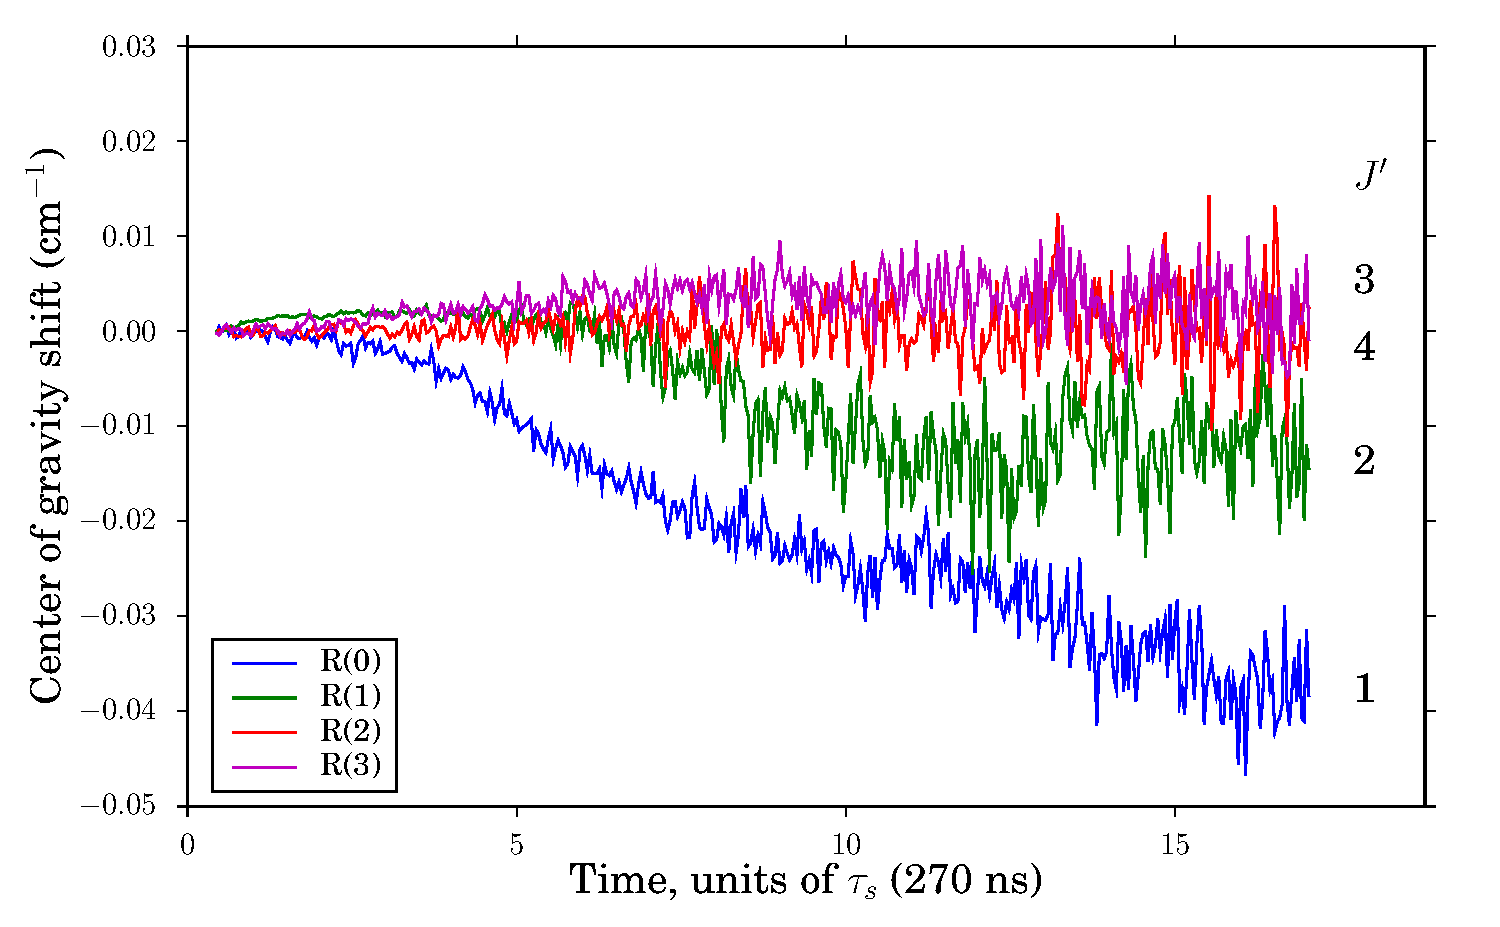
\includegraphics[width=6in]{2231-r0123-cog-delay.pdf}
% \end{figure}

% %%%%%%%%%%%%%%%%%%%%%%%%%%%%%%%%%%%%%%%%%%%%%%%%%%%%%%
% %%
% %% END OF 2^2 3^1 FIGURES
% %%
% %%%%%%%%%%%%%%%%%%%%%%%%%%%%%%%%%%%%%%%%%%%%%%%%%%%%%%

% Although the $2^23^1$ \Ka{1} sublevel has the highest energy of the
% four sublevels in this study, it interacts most weakly with the local
% manifold of $T_{1,2}$ levels.  This results from having only one
% quantum of the $\nu_3$ vibration, which controls the overall magnitude
% of $S_1 \sim T_3$ doorway matrix elements.

% The spectrum of the $2^23^1$ \Ka{1} $\leftarrow$ $0_0$ subband is
% shown in Figure \ref{fig:spectrum-2231}.  Besides the overall
% SEELEM:LIF intensity ratio, the small magnitude of $S_1 \sim T_3$
% doorway matrix elements is indicated by the width of the SEELEM
% intensity envelope surrounding each singlet transition.  This topic is
% discussed at length in Chapter 2.  Briefly, the width of the SEELEM
% spectrum is a measure of the energy range over which the singlet
% level, through interaction with $T_3$ doorways, is able to lend
% approximately 0.25\% fractional singlet character within the local
% manifold of $T_{1,2}$ levels.  In the case of $2^23^1$ \Ka{1}, the
% width of the SEELEM envelope surrounding each singlet transition is on
% the order of 0.4 \rcm, much less than the average spacing between
% rotational lines.  In the next section, we will contrast this with the
% observed width of SEELEM intensity envelopes in a strongly interacting
% subband.

% % Using a formula
% % derived in Chapter 2, the FWHM of the SEELEM spectrum can be related
% % to the $S_1 \sim T_3$ doorway matrix element, $H_{S_1,T_3}$, and the
% % average $T_3 \sim T_{1,2}$ matrix element, $\braket{H_{T_3,T_{1,2}}}$:
% % \begin{equation}
% %   \Delta E_{FWHM} = \frac{2\sqrt{2} \; \tau_s}
% %                        {e \; \tau_{\text{flight}}}
% %   \left \lvert
% %     \frac{H_{S_1,T_3} \braket{H_{T_3,T_{1,2}}}}{\Delta E_{S_1,T_3}}
% %   \right \rvert,
% % \end{equation}
% % where $\Delta E_{S_1,T_3}$ is the energy difference between the
% % singlet level and the $T_3$ doorway, and $\tau_{\text{flight}}$ is the
% % flight time in the SEELEM apparatus, about 310 \microsec.  Solving for
% % the quantity $\lvert H_{S_1,T_3} \braket{H_{T_3,T_{1,2}}} / \Delta
% % E_{S_1,T_3} \rvert$ and using the approximate FWHM of 0.4 \rcm, we
% % find that
% % \begin{equation}
% % \end{equation}

% The dependence of the intensity-weighted center of gravity for each
% transition in $2^23^1$ \Ka{1} is shown in Figure
% \ref{fig:2231-cog-delay}.  With the exception of the Q(1) and R(0)
% transitions, the center of gravity does not deviate by more than 0.02
% \rcm\ from the initial position.  For a level having such a small
% matrix element, any small change in center of gravity which might arise
% from the effects of an energetically distant $T_3$ level is not
% expected to appear until delay times in excess of $15\tau_s$.

% The anamalous behavour of the center of gravity for the Q(1) and R(0)
% transitions is once again evidence of a weak, local $T_3$ perturbation
% at $J'=1$.  The upper states of the Q(1) and R(0) transitions have the
% same $J'$, but differ in parity (being of $f$- and $e$-symmetry,
% respectively).  The energy difference between the \emph{e}- and
% \emph{f}-symmetry components is $\Delta E_{e-f}=+0.13$ \rcm.  The
% perturbation in the \emph{e}-symmetry singlet transition R(1) is to
% lower energy, with a magnitude of approximately $-0.03$ \rcm, while
% the perturbation in the \emph{f}-symmetry singlet level is to lower
% energy, with a magnitude of approximately $+0.03$ \rcm.  The splitting
% between the asymmetry components of the $T_3$ perturber is therefore
% less than $0.13-0.03-0.03=0.07$ \rcm at $J'=1$.  An asymmetry
% splitting of this magnitude would be unusually small for a $T_3$ level
% with $K_T=1$.  As a result, we conclude that the perturber is likely a
% level with $K_T=2$.  Only one component of a $K_T=2$ level may
% interact with a singlet level at $J'=1$, and that is the $F_3$
% component, where $N_T=J+1$.  An interaction with the $F_1$ or $F_2$
% components would require $N_T$ to be $0$ or $1$; these levels are not
% present when $K_T=2$.  Because the interaction occurs via the $F_2$
% component of the triplet level at $J'=1$, the rotationless energy of
% the triplet level must be approximately $4B \simeq 4$ \rcm\ to the red
% of the singlet level.

% Again, the assignment of the $K_a$ quantum number for a $T_3$ level
% observed in the spectrum has allowed us to infer its energy relative
% to the singlet.  At $J'=2$, the nearest component of this weak $T_3$
% perturber is $2B \simeq 2$ \rcm\ above the singlet level.  The
% resultant increase in squared energy denominator makes the
% perturbation $(2.0/0.03)^2 \simeq 4500$ times weaker at $J'=2$, and it
% is not observed.

% %
% % Selection rules: Q   -> e-f
% %                  P,R -> e-e, f-f
% % 











% \subsection{The $3^3$ \Ka{2} sublevel: spectral patterns in the
%   presence of large $S_1 \sim T_3$ matrix elements}

% % Spectrum:  Jan 22C, p.31,34 of 1/2007--3/2007 notebook.

% %%%%%%%%%%%%%%%%%%%%%%%%%%%%%%%%%%%%%%%%%%%%%%%%%%%%%%
% %%
% %% INSERT 3^3 K^2 FIGURES HERE
% %%
% %%%%%%%%%%%%%%%%%%%%%%%%%%%%%%%%%%%%%%%%%%%%%%%%%%%%%%

% \begin{figure}
%   \caption{Simultaneously recorded SEELEM (upper trace) and LIF (lower
%     trace) spectra of the $3^3$ \Ka{2} sublevel of the \astate\ state
%     of \ce{C2H2}.  The LIF spectrum is integrated in two time regions:
%     an early time window ($0.5\tau_s-2\tau_s$, solid trace) and a
%     delayed time window ($10\tau_s-18\tau_s$, dashed trace).  The
%     individual transitions are each split at least two strongly mixed
%     components.  Although the energy splitting between the components
%     is on the order of the experimental resolution, they are
%     discernable via changes in the fluorescence lineshape resulting
%     from their differing relative intenities in the early and delayed
%     fluorescence spectra.  One splitting in the R(4) transition is
%     just resolved in this spectrum.  \TODO{Determine the assignment
%       for the set of overlapping transitions.}}
%   \label{fig:spectrum-33k2}
%   \centering
%   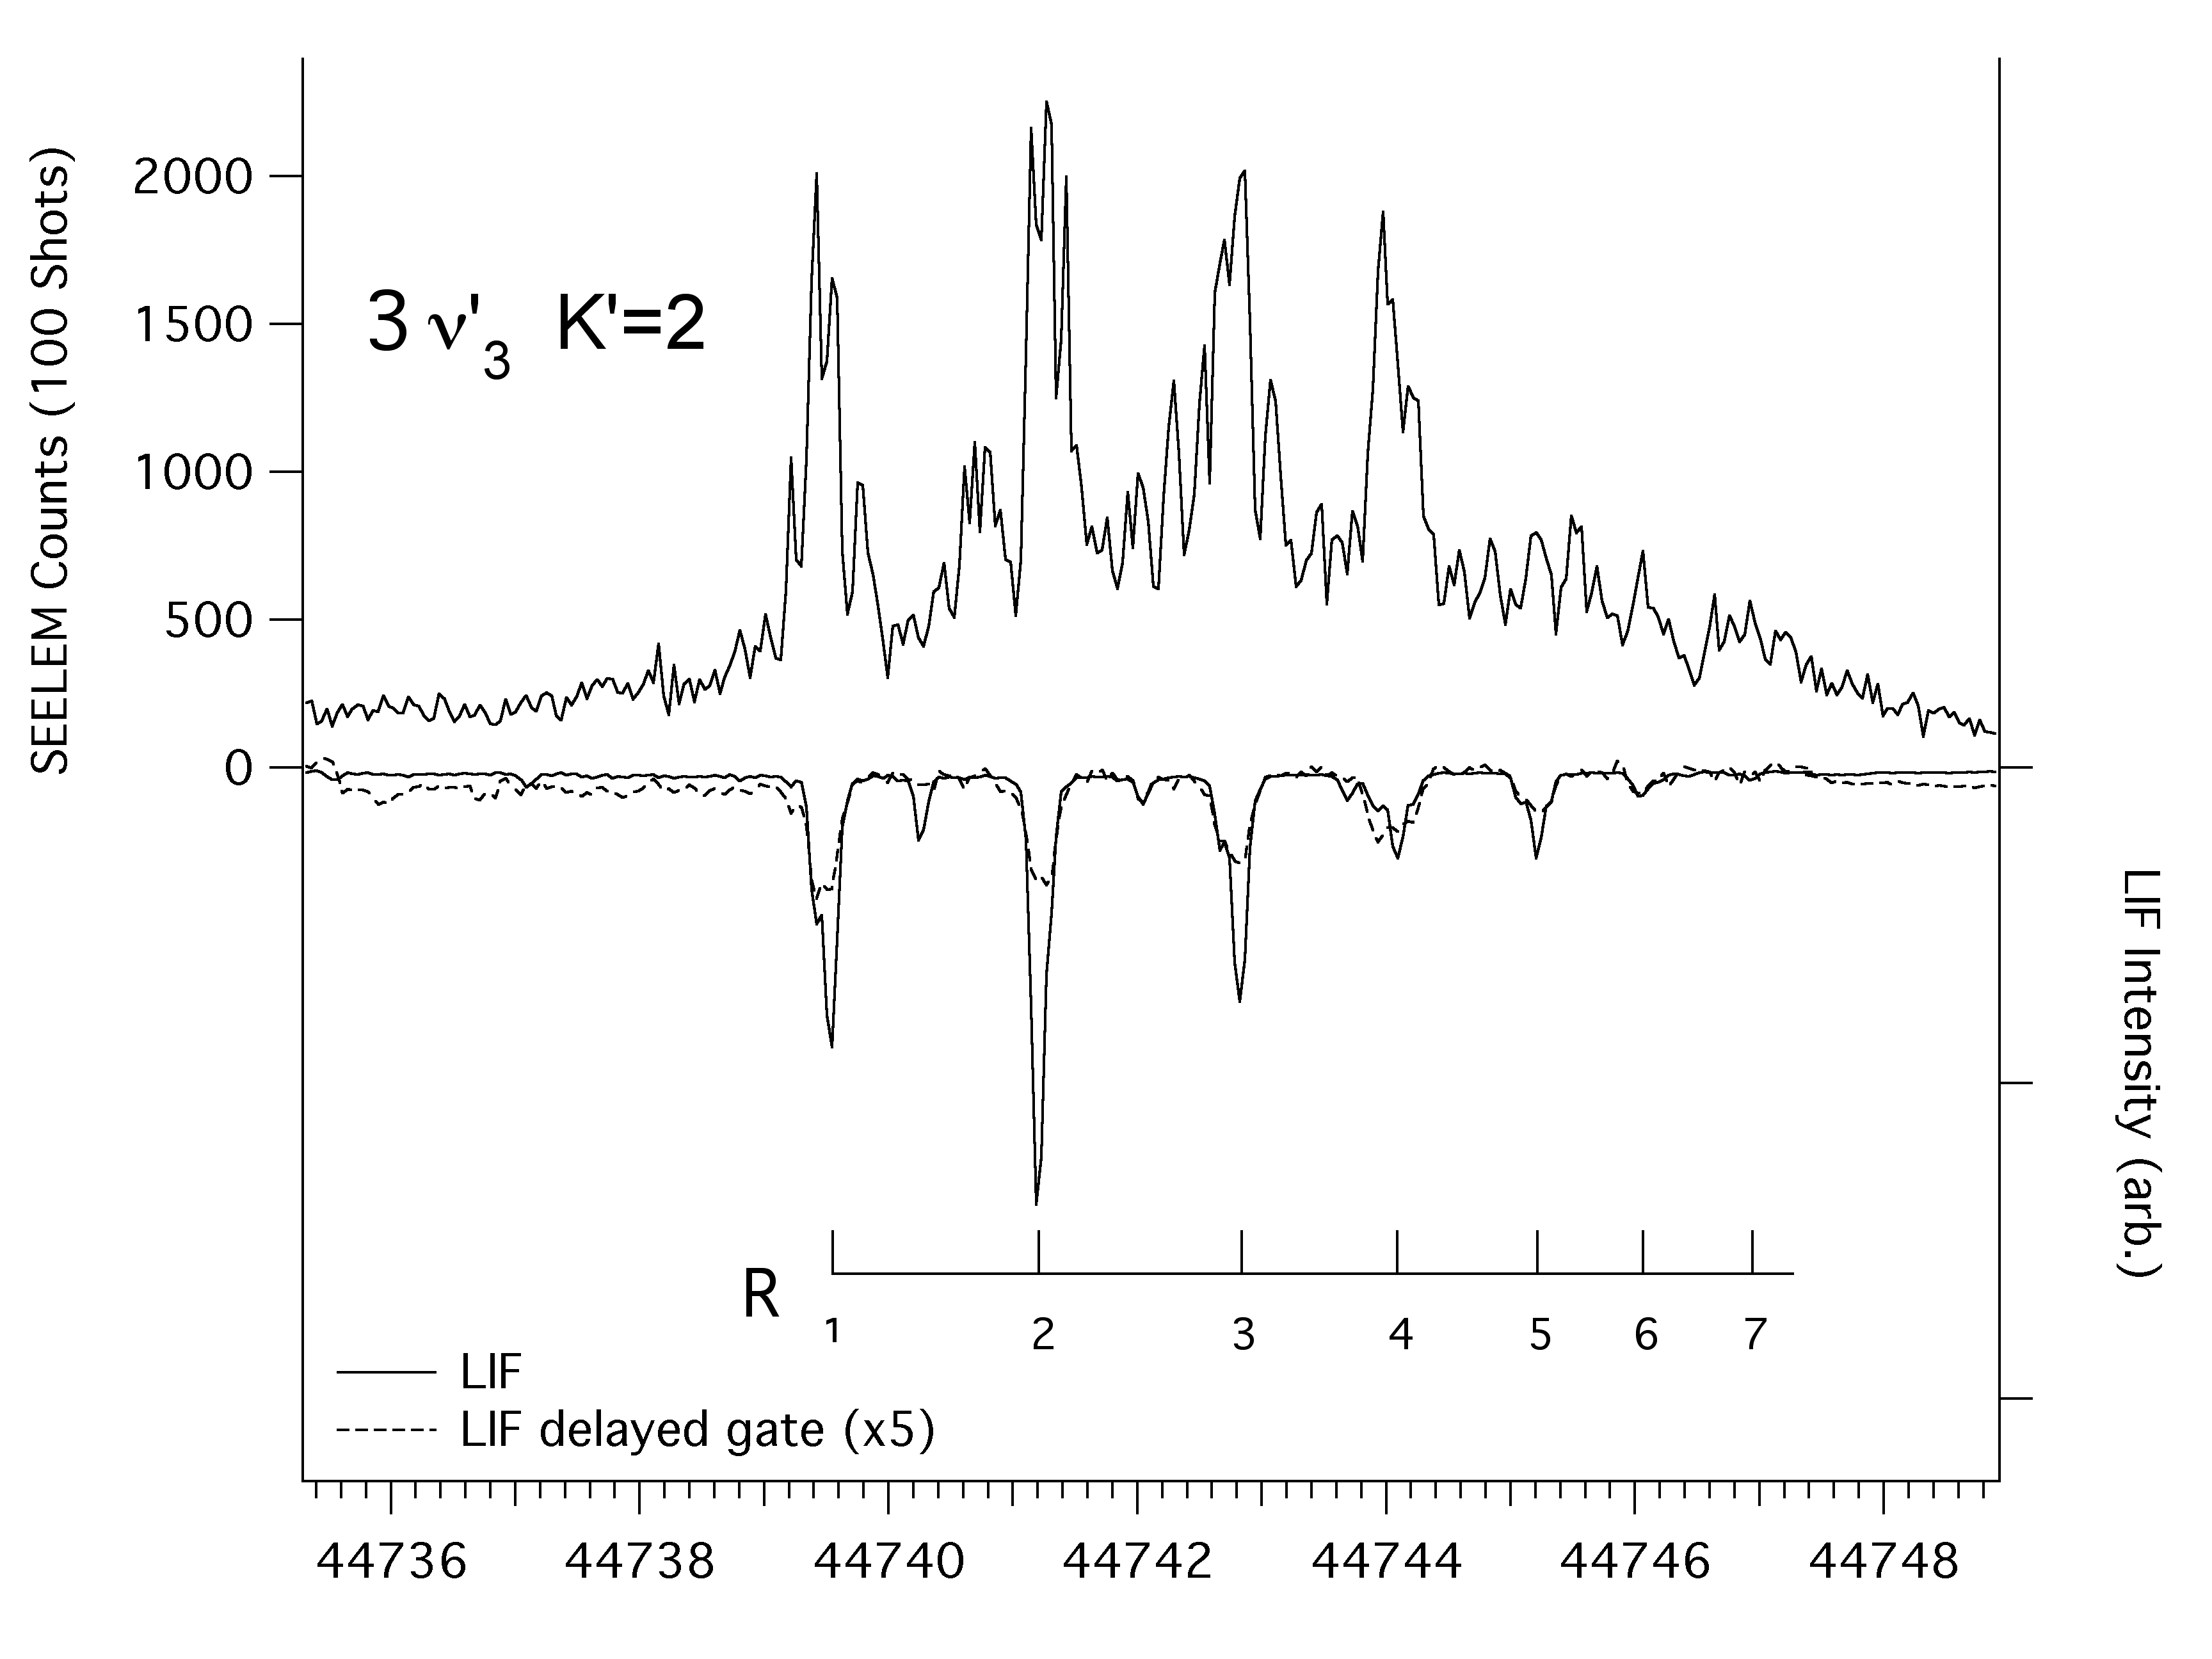
\includegraphics[width=7in,angle=90]{acetylene-33k2-r1r7.png}
% \end{figure}

% \begin{figure}
%   \caption{Dependence of the intensity-weighted center of gravity on
%     delay for a series of individually resolved transitions, R(1$-$7),
%     in the LIF spectrum of the $3^3$ \Ka{2} sublevel.  The individual
%     transitions have an overall bias to lower energies at long delay
%     times, indicating an interaction with a $T_3$ doorway level at
%     lower energy.}
%   \label{fig:33k2-cog-delay}
%   \centering
%   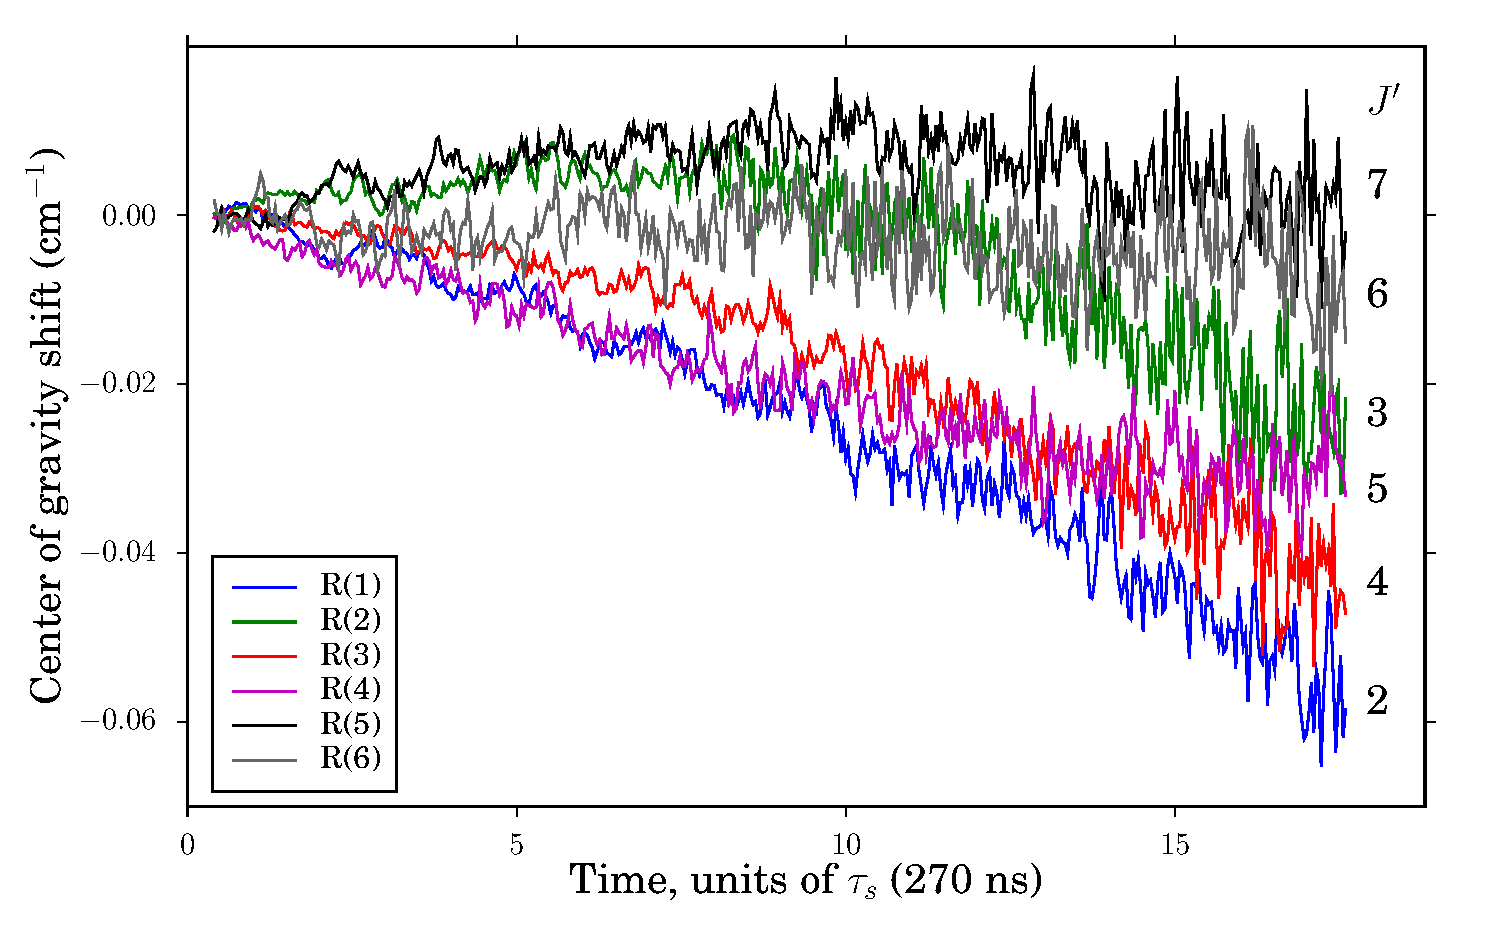
\includegraphics[width=6in]{33k2-r123456-cog-delay.pdf}
% \end{figure}

% %%%%%%%%%%%%%%%%%%%%%%%%%%%%%%%%%%%%%%%%%%%%%%%%%%%%%%
% %%
% %% END OF 3^3 K^2 FIGURES
% %%
% %%%%%%%%%%%%%%%%%%%%%%%%%%%%%%%%%%%%%%%%%%%%%%%%%%%%%%

% The $3^3$ \Ka{2} sublevel is the higher-energy sibling of $3^3$
% \Ka{1}, which has been studied in great detail due to a large
% perturbation from a $T_3$ doorway level with matrix element $\simeq
% 0.1$ \rcm.  The $T_3$ pertuber observed in $3^3$ \Ka{1} has been
% assigned as the $F_2$ component of $K_T=1$, because 
% %\begin{inparaenum}[\itshape a\upshape)]
% %\item 
% it tunes slowly with energy,
% %\item 
% it interacts with both parities of the singlet, and
% %\item 
% the perturbation is present at $J'=1$
% %\end{inparaenum}
% \cite{mishra04}.  It has been suggested that the $K_T=0$ sublevel of
% this perturber is responsible for the large Zeeman anticrossing
% observed in $3^3$ \Ka{0} \cite{thom07, dupre93}.  To account for this,
% the $A$-rotational constant of the perturbing $T_3$ level would have
% to closely match the constant for the singlet level.  However, it is
% highly improbable that an energetic near match in the $K_a=0$ and $1$
% sublevels, separated by $1A \simeq 15$ \rcm, will extend to $K_a=2$,
% which is $3A \simeq 45$ \rcm\ higher in energy.  In the absence of a
% local $T_3$ perturbation, the $3^3$ \Ka{2} sublevel provides an
% excellent opportunity to look examine a singlet sublevel which is
% known to be capable of large vibrational overlap with $T_3$ levels.

% The $3^3$ \Ka{2} sublevel is not accessible from the ground state of
% acetylene due to $\Delta K = \pm 1$ selection rules.  However, the
% spectrum of the $3^3$ \Ka{2} $\leftarrow$ $4_1$ ``hot band''
% transition could be taken with appreciable signal to noise in our
% apparatus without heating the nozzle.  The simultaneously recorded
% SEELEM and LIF spectrum the R-branch of this transition is shown in
% Figure \ref{fig:spectrum-33k2}.  Another interloping transition is
% present in the spectrum with low intensity, giving rise to the weak
% lines at 44740.3, 44742.2, and 44743.6 \rcm.  No intensity alternation
% is present in the rotational series, as expected in a band which
% originates from the $4^2$ vibrational level of the ground electronic
% state.

% Evidence of strong mixing with the local manifold of $T_{1,2}$ levels
% is present in both the SEELEM and LIF detection channels.  The SEELEM
% intensity envelope surrounding each singlet transition exceeds the
% spacing between adjacent rotational lines, about 1.5 \rcm at low $J'$.
% This is at least 4 times the width observed for the transitions in
% $2^23^1$ \Ka{1}, which contains only quantum of excitation in $\nu_3$.
% The increased width of the local SEELEM intensity envelope has the
% effect of creating a cumulative intensity envelope extending across
% the entire spectrum.  This effect is also observed in the $3^3$ \Ka{1}
% $\leftarrow$ $0_0$ spectrum (see reference \cite{humphrey97}, for
% example).  However, in $3^3$ \Ka{2}, no interference effects are
% observed in SEELEM, which would indicate a $T_3$ doorway level
% crossing.

% Splittings are evident in the LIF spectrum of each transition, even in
% the early time-gated LIF spectrum.  Splittings which are slightly
% below the laser resolution can be seen due to the different relative
% intensities of long and short lifetime components in the early and
% delayed LIF spectra.  Two of three strong components are resolved in
% the early LIF spectrum of the R(4) transition.  No such splittings are
% present in the weakly interacting $2^23^1$ \Ka{1} sublevel.

% % An estimation of the
% % effective, $T_3$-mediated $S_1 \sim T_{1,2}$ average matrix element
% % can be made by the fact that nearly every singlet level is able to
% % donate fractional singlet character of approximately 10\% to a local
% % $T_{1,2}$ level approximately 0.06 \rcm\ away in energy.  Dividing the
% % square root of the mixing fraction by the energy denominator gives an
% % approximate matrix element of 

% The dependence of the intensity-weighted center of gravity for each
% transition in $3^3$ \Ka{2} is shown in Figure
% \ref{fig:33k2-cog-delay}.  The transitions display an overall bias to
% lower energy, indicating a $T_3$ doorway level to lower energy.  The
% $F_3$ components of such a doorway level would approach the singlet
% level from below at a rate of $2B$ per $J'$, while the $F_2$
% components would remain energetically distant and the $F_1$ components
% would rapidly tune away.  That no crossing is observed by at least
% $J'=6$ means that the doorway must be at least $6\times2B + 2B \simeq
% 14$ \rcm\ lower in energy than the singlet level.

% The center of gravity changes with the greatest magnitude for the
% $J'=2$ rotational level, and the magnitude of shift generally
% decreases with $J'$.  However, if the $F_3$ component of the doorway
% level is rapidly approaching the singlet, the overall coupling is
% expected to increase.  Why does the magnitude of the change in center
% of gravity not also increase?  This apparent paradox is explained by
% the great amount of fractional singlet character in nominal $T_{1,2}$
% levels, which is induced by strong coupling to the doorway.  As
% several components of nominal $T_{1,2}$ electronic character borrow
% more intensity, their lifetime decreases.  As the nominal singlet
% level lends out more fractional character, its lifetime increases.
% The result is a lack of contrast between the intensities of the
% nominal singlet and nominal triplet eigenstates as a function of delay
% time, resulting in a smaller changes in the intensity-weighted center
% of gravity.

% However, evidence for the approach of energetically distant $T_3$
% doorway levels is still available from the spectrum.  The most
% reliable indicator is a comparison of band-integrated center of
% gravity of the early LIF spectrum vs. the SEELEM spectrum.  We discuss
% this in the following section.

% \subsection{Evidence for energetically distant $T_3$ doorway levels in
%   band-integrated center-of-gravity}

% %%%%%%%%%%%%%%%%%%%%%%%%%%%%%%%%%%%%%%%%%%%%%%%%%%%%%%
% %%
% %% INSERT CENTER-OF-GRAVITY TABLE HERE
% %%
% %%%%%%%%%%%%%%%%%%%%%%%%%%%%%%%%%%%%%%%%%%%%%%%%%%%%%%

% \begin{table}
%   \caption{Band-integrated center of gravity measurements from
%     simultaneously recorded SEELEM/LIF spectra of \astate\ acetylene.
%     The SEELEM$-$LIF center of gravity is offset to lower energy for
%     Q-branch measurements and offset to higher energy for R-branch measurements, 
%     indicating an overall increase in relative SEELEM:LIF intensity
%     with $J'$.  Such $J'$-dependent behavior is predicted in the
%     presence of energetically distant $T_3$ doorway levels.}
%   \label{table:integrated-cog-shifts}

%   \centering
%         \begin{tabular}{lllll}
%         \\[1cm]
%         \multicolumn{3}{l}{Q-branch measurements} \\
%         \toprule
%         Level & Integration region & \multicolumn{2}{l}{Center of gravity} & Offset \\
%         \cmidrule{3-5}
%         & & LIF & SEELEM & SEELEM$-$LIF \\
%         \midrule
%         $\nu'_2+2\nu'_3$ & 45671.75$-$76.30 & 45674.60 & 45674.09 & $-0.51$ \\
%         $2\nu'_2+\nu'_3$ & 46004.50$-$08.50 & 46007.29 & 46007.23 & $-0.06$ \\
%         $2\nu'_3+2\nu'_4$ & 45807.30$-$11.00 & 45810.09 & 45809.72 & $-0.37$ \\
%         \bottomrule
%         \end{tabular}

%         \begin{tabular}{lllll}
%         \\[1cm]
%         \multicolumn{3}{l}{R-branch measurements} \\
%         \toprule
%         Level & Integration region & \multicolumn{2}{l}{Center of gravity} & Offset \\
%         \cmidrule{3-5}
%         & & LIF & SEELEM & SEELEM$-$LIF \\
%         \midrule
%         $2\nu'_2+\nu'_3$ & 46009.50$-$16.50 & 46012.11 & 46012.49 & $+0.38$ \\
%         $3\nu'_3 \:\; K'\!=\!2$ & 44738.50$-$47.50 & 44741.79 & 44742.67 & $+0.88$ \\
%         $2\nu'_3+2\nu'_4$ & 45812.00$-$20.50 & 45814.67 & 45815.57 & $+0.89$ \\
%         \bottomrule
%         \end{tabular}
% \end{table}

% %%%%%%%%%%%%%%%%%%%%%%%%%%%%%%%%%%%%%%%%%%%%%%%%%%%%%%
% %%
% %% END CENTER-OF-GRAVITY TABLE
% %%
% %%%%%%%%%%%%%%%%%%%%%%%%%%%%%%%%%%%%%%%%%%%%%%%%%%%%%%

% \NOTE{Just the table for now.}





























% \section{Conclusion}

% The mechanism of doorway-mediated coupling by an energetically distant
% $T_3$ level skews the coupling to the local $T_{1,2}$ states that
% appear in the SEELEM spectrum, resulting in a center-of-gravity shift
% between the LIF and SEELEM spectra.  Additionally, when viewed in
% successive time windows, the center of gravity of the LIF spectrum
% exhibits evolution toward the limiting behavior exhibited in the
% SEELEM spectrum.  A simple model can be used to show that strong
% coupling between the singlet level and the mediating $T_3$ level
% causes a gradual shift in the center of gravity, while weak coupling
% to the mediating level induces a more delayed and rapid shift in the
% center of gravity, with respect to the bright state lifetime.

% Rotational selection rules for $S_1 \sim T_3$ spin-orbit coupling give
% rise to $J$-dependent effects in the LIF/SEELEM spectrum.  As $J$
% increases, the $\Delta N$= +1 or -1 components of any distant $T_3$
% level approach the singlet at a rate $d\Delta E / dJ$ of approximately
% $2B_T$ ($\sim$2 \rcm\ per $J$).  In the spectrum, the result is a
% shift in the LIF-SEELEM center of gravity when integrated across an
% entire branch of transitions.  The effect not only leads to strong
% $J$-dependent changes in the patterns of $T_3$-mediated coupling, but
% also ensures detection and assignment of $S_1 \sim T_3$ level
% crossings at relatively low values of $J$.

% % \POINT{The LIF/SEELEM spectra for the progression of $2^n3^m$ levels
% %   shows the expected trends for strong coupling.}

% \POINT{For every $S_1$ vibrational level, a $T_3$ doorway level is
%   rapidly approaching with $J$.}  Because of this, further LIF/SEELEM
% spectroscopy of the acetylene \AtoX\ transition will be fruitful and
% informative.  We highlight some candidates for future investigation.
% \begin{enumerate}
% \item Levels which exhibit long lifetimes or quantum beats in the LIF
%   spectrum
% \item levels with unassigned perturbations or splittings,
% \item other $3^2B^2$ polyad members
% \item other $K$-sublevels of the Franck-Condon active levels studied
%   here.  
% \end{enumerate}
% \TODO{Specify candidate bands specifically, give energies.}

% \POINT{Outline prospects for studying quantum beats in tandem with
%   delayed fluorescence and SEELEM.}  The appearance of population
% quantum beats in the spectrum indicates a splitting on the order of 80
% MHz or less.  Quantum beat waveforms follow a well-defined form, and
% an analysis of quantum beats determines both the matrix element and
% zero-order energy spacing of the levels involved.  The matrix elements
% gained from an analysis of zero-field quantum beats in the acetylene
% spectrum can serve as a probe of the magnitude of
% local matrix elements between the nominal $S_1$ bright state and
% neighboring $T_{1,2}$ dark states.  Furthermore, the study of Zeeman
% quantum beats at low magnetic fields can provide a method for
% distinguishing between triplet perturbations and perturbations from
% other singlet levels, such as $S_1$ levels which are localized in the
% \emph{cis} geometry of the \astate\ state.

\bibliography{master} 
\bibliographystyle{plain}
\end{document}
% LocalWords:  redshifted blueshifted sublevel pdf png



President's Report:

The T_3 electronic state is peculiar among the valence states of
acetylene due to its out-of-plane equilibrium geometry. One of the
most interesting unsolved problems in the intersystem crossing of
acetylene is the role of the non-symmetric in- and out-of-plane S_1
bending modes (\nu_4 and \nu_6) in promoting coupling to the nonplanar
T_3 state.  To investigate this issue, we have used an IR-UV-Double
Resonance technique to record simultaneous LIF/SEELEM spectra of the
3^3 4^1 K=0 and 3^3 6^1 K=0 levels.  This method allows us to record
the spectrum of weakly coupled T_1,2 levels without overlap from
adjacent rotational transitions.

[Additionally, we have used a polarization technique in tandem with
IRUVDR to record the spectrum of the rotationless level in 3^3 6^1
K=0.  Due to spin-orbit selection rules, only triplet levels having
K_T = J_T = N_T = 0 may appear in the spectrum -- thus, the local
T_1,2 level density may be obtained from a direct count of SEELEM
transitions.]


That should be K_T = J_T = 0 and N_T = 1...my bad. For a K=0 triplet
level in Hund's case (b),

N            J

  ---------- 3
2 ---------- 2
  ---------- 1


  ---------- 2
1 ---------- 1
  ---------- 0  ***


0 ---------- 1

--Kyle



The total spin-orbit matrix element between a rovibronic level of S_1
and a level of T_3 is the product of an electronic factor, a
vibrational overlap factor, and a rotational factor (arising from
angular momentum coupling laws).

OK, these are kind of hairy, but hold on before you start to panic.
As it turns out, the energy differences between levels of S_1 and T_3
vary much more rapidly than the rotational factors.  This is due to
the spin-orbit selection rule of \Delta_N = 0, +1, -1.

Take a look at this plot: It shows the relative energies of the three
triplet rotational components that are connected to singlet level: F_1
(\Delta_N = -1), F_2 (\Delta_N = 0), and F_3 (\Delta_N = +1).  This
plot is made in the approximation that the singlet and triplet
B-values are nearly equal.  Imagine placing a singlet level at some
energy on the plot - the energy of the singlet could be represented by
a horizontal line.  If the singlet is very close to zero, the F_2
component varies slowly with rotation and the F_1,2 components rapidly
speed away.  Essentially, only the F_2 component matters when J>1.

If the singlet is not located close to zero, EITHER the F_1 or the F_3
component of the triplet is rapidly approaching.  The triplet
component approaches with a rate of about 2 cm-1 per rotational
quantum number. According to Ryan and Bryan's calculations, the
<electronic*vibrational> spin-orbit matrix elements between S_1 and
T_3 max out at about 0.1 cm-1. The rotational factor only reduces this
value.  Compared to the matrix element, an energy difference of 2 cm-1
per J is huge!

I believe that strongly coupled, mediating T_3 levels will make
themselves known at several values of J through this
energy-denominator effect.  I think this is what we observe in our 3^3
K=2 data.  Weakly coupled T_3 levels should appear as perturbations at
a single J, and then immediately disappear, because their matrix
elements are much, much less than 2 cm-1. This means that weak triplet
perturbations should be _common_, and it means that we should be able
to infer their approximate energy from the value of J which is
perturbed in the singlet, i.e. + or - (J*2*B).

This means that further SEELEM spectroscopy of the S_1 state should be
fruitful and informative.  I hope you are all totally stoked!  I'll
discuss the experimental consequences and possibilities in a later
email.

--Kyle
